\chapter{Appendices}

\section{Strategies for the reiterated Prisoner's Dilemma}

In the following subsections all strategies that occur in the reiterated two
person Prisoner's Dilemma simulations in chapter \ref{modeling} will be
described. In subsection \ref{ordinaryStrategies} all of the strategies that
were used in the first simple model of reciprocal altruism (see chapter
\ref{simpleModel}) will be described. The following subsections
\ref{parameterizedTFTs} and \ref{twoStateAutomata} explain the strategies that
were used in the simulation series of chapter \ref{refinedModel}. Finally,
subsection \ref{signalingCheaters} describes the family of {\em Signaling
  Cheater}-strategies plus the strategy {\em Signaling Cheater}, a member of
which was used in the group selection scenario in chapter
\ref{groupSelectionContraAltruism}. The verbal description of the strategies
is supplemented by their implementation in the {\tt Python} programing
language. For the better understanding of the program code, it should be kept
in mind that a return value of one signifies a cooperative move, while a
return value of zero translates into a defective move in the game.

\subsection{Ordinary strategies}
\label{ordinaryStrategies}

Following is a description of the strategies that were used for the ``simple
model'' of chapter \ref{simpleModel}.

\paragraph{Tit for Tat} The strategy {\em Tit for Tat} starts with a
cooperative move in the first round. In the subsequent rounds {\em Tit for
Tat} cooperates if the other player cooperated in the previous rounds. If the
other player defected in the previous round, {\em Tit for Tat} punishes the
defector by defecting itself.
\begin{scriptsize}
\begin{verbatim}
class TitForTat(Strategy):
    def firstMove(self):
        return 1             # cooperate in the first round
    def nextMove(self, myMoves, opMoves):
        return opMoves[-1]   # reciprocate opponent's last move
\end{verbatim}
\end{scriptsize}

\paragraph{Grim} The strategy {\em Grim} starts with a cooperative move and
continues to cooperate unless the other player defects. Once the other player
has failed to reciprocate cooperation {\em Grim} defects unanimously throughout
the remainder of the game.
\begin{scriptsize}
\begin{verbatim}
class Grim(Strategy):
    def firstMove(self):
        self.punish = False
        return 1
    def nextMove(self, myMoves, opMoves):
        if self.punish:  return 0
        elif opMoves[-1] == 1:  return 1  
        else:
            self.punish = True
            return 0
\end{verbatim}
\end{scriptsize}

\paragraph{Dove} The strategy {\em Dove} always cooperates, no matter what the
other player does.
\begin{scriptsize}
\begin{verbatim}
class Dove(Strategy):
    def firstMove(self):
        return 1
    def nextMove(self, myMoves, opMoves):
        return 1
\end{verbatim}
\end{scriptsize}

\paragraph{Hawk} The strategy {\em Hawk} never cooperates.
\begin{scriptsize}
\begin{verbatim}
class Hawk(Strategy):
    def firstMove(self):
        return 0
    def nextMove(self, myMoves, opMoves):
        return 0
\end{verbatim}
\end{scriptsize}

\paragraph{Random} The strategy {\em Random} cooperates or defects at random
with a 50\% chance.
\begin{scriptsize}
\begin{verbatim}
class Random(Strategy):
    def firstMove(self):
        return random.randint(0,1)
    def nextMove(self, myMoves, opMoves):
        return random.randint(0,1)
\end{verbatim}
\end{scriptsize}

\paragraph{Tester} The strategy
{\em Tester} starts off with two defections. If the opponent does not answer
these defections with punishment, {\em Tester}
classifies the opponent as an exploitable strategy and defects every second
round during the remainder of the match. Otherwise {\em Tester} tries
to appease the other player with two cooperative moves in round three and
four and then switches to the fairly reliable strategy {\em Tit for Tat} for
the remainder of the reiterated game.
\begin{scriptsize}
\begin{verbatim}
class Tester(Strategy):
    def firstMove(self):
        self.state = "Test"
        return 0
    def nextMove(self, myMoves, opMoves):
        if self.state == "Test":
            self.state = "Evaluate"
            return 0
        elif self.state == "Evaluate":
            if opMoves[-1] == 0:
                self.state = "Consolation"
                return 1
            else:
                self.state = "Dove"
                return 0
        elif self.state == "Consolation":
            self.state = "TitForTat"
            return 1
        elif self.state == "Dove":
            self.state = "Hawk"
            return 1
        elif self.state == "Hawk":
            self.state = "Dove"
            return 0
        elif self.state == "TitForTat":
            return opMoves[-1]
        else:
            raise AssertionError, \
                  "Tester: state %s is not a valid state!"%self.state
\end{verbatim}
\end{scriptsize}

\paragraph{Pavlov} Named after the famous Russian physiologist who discovered
the ``conditional reflex'', the strategy {\em Pavlov} plays ``win stay, lose
shift'', starting with a defection. Other than for example {\em Tit for Tat} it
will continue with defecting, if the opponent fails to punish defections.
\begin{scriptsize}
\begin{verbatim}
def invertMove(move):
    """--> inverted move. (0 becomes1 and 1 becomes 0)"""
    if move == 0:  return 1
    else:  return 0
class Pavlov(Strategy):
    def firstMove(self):
        self.condition = 0
        return self.condition
    def nextMove(self, myMoves, opMoves):
        if opMoves[-1] == 0:
            self.condition = invertMove(self.condition)
        return self.condition
\end{verbatim}
\end{scriptsize}

\paragraph{Tranquilizer} The strategy {\em Tranquilizer} is a refinenement of
the strategy ``Tit for two tats'' which usually cooperates and only punishes
the opponent with a defection if the opponent has defected during the two
previous rounds. But in contrast to ``Tit for two tats'', {\em Tranquillizer}
also defects unmotivated with a random probability that increases during the
course of the repeated game. (This reflects the consideration that good
relations with the other player become less important the shorter the shadow
of the future is.) The random defection probability is zero in the beginning
and is increased by 1\% before each round, up to a limit of 50\%.
\begin{scriptsize}
\begin{verbatim}
class Tranquilizer(Strategy):
    def firstMove(self):
        self.evilFactor = 0.0
        return 1
    def nextMove(self, myMoves, opMoves):
        if self.evilFactor < 0.5:  self.evilFactor += 0.01
        if opMoves[-2:] == [0,0]:
            return 0
        else:
            if random.random() < self.evilFactor: return 0
            else:  return 1
\end{verbatim}
\end{scriptsize}

\paragraph{Joss} The strategy {\em Joss} basically plays ``Tit for tat'', but
it defects unmotivated (i.e.\ in cases where it does not defect to punish the
opponent for a defection in the previous round) with a random probability of
10\%.
\begin{scriptsize}
\begin{verbatim}
class Joss(Strategy):
    def firstMove(self):
        return 1
    def nextMove(self, myMoves, opMoves):
        if opMoves[-1] == 0:  return 0
        else:
            if random.random() < 0.1:  return 0
            else:  return 1
\end{verbatim}
\end{scriptsize}

\newpage

\subsection{Parameterized {\em Tit for Tat}-strategies}
\label{parameterizedTFTs}

The {\em Parameterized Tit for Tat}-strategies are derived from {\em Tit for
Tat} by adding the two parameters {\em good
rate} and {\em evil rate} to modify the behavior of {\em Tit for Tat}.
The {\em good rate} is a probability with which the {\em Parametrized Tit
for Tat} makes a cooperative move when the ordinary {\em Tit for Tat}
would not. And, conversely, the {\em evil rate} defines a probability with
which the parametrized strategy defects when normally {\em Tit for Tat}
would cooperate. If both the {\em good rate} and the {\em evil rate} are
zero then the {\em Parametrized Tit for Tat}-strategy is the same as the
ordinary {\em Tit for Tat}. If the {\em good rate} is 1 and the evil rate is
0 then it is the same as {\em Dove}. If, conversely, the {\em evil rate} is
1 and the {\em good rate} is 0 then then strategy played is the same as {\em
Hawk}. If both rates are 0.5 it is the same as the {\em Random}-strategy.

The implementation of the {\em Parameterized Tit for Tat}-strategies below
takes account of these connections by appending appropriate suffixes to the
name of the strategy in these special cases. The names of the {\em
  Paramterized Tit for Tat}-strategies consist of the ``family name'', which
is ``P\_TFT'' followed by the goodrate and the evil rate and possibly by a
suffix to indicate a meaningful speacial case. Thus ``P\_TFT 0.2 0.4'' is the
name of the {\em Parameterized Tit for Tat}-strategy with a {\em good rate} o
f 20\% and an {\em evil rate} of 40\%, while ``P\_TFT 0.5 0.5 (Random)'' names
the {\em Parameterized Tit for Tat} strategy with both a {\em good-} and {\em
  evil rate} of 50\%, which is in effect the {\em Random}-strategy.

\begin{scriptsize}
\begin{verbatim}
class ParameterizedTFT(Strategy):
    def __repr__(self):
        return self.__class__.__name__ + "(" + repr(self.goodrate) + \
               ", " + repr(self.evilrate) + ")"
    def __init__(self, goodrate=0.2, evilrate=0.05):
        assert goodrate >= 0.0 and goodrate <= 1.0, "goodrate must be >= 0 and
<= 1!"
        assert evilrate >= 0.0 and evilrate <= 1.0, "evilrate must be >= 0 and
<= 1!"
        Strategy.__init__(self)
        self.randomizing = True
        self.goodrate = goodrate
        self.evilrate = evilrate
        self.name = "P_TFT %1.2f %1.2f" % (self.goodrate,self.evilrate)
        if self.goodrate == 1.0 and self.evilrate == 0.0:
            self.name += " (Dove)"
        elif self.evilrate == 1.0 and self.goodrate == 0.0:
            self.name += " (Hawk)"
        elif self.goodrate == 0.0 and self.evilrate == 0.0:
            self.name += " (TitForTat)"
        elif self.goodrate == 0.5 and self.evilrate == 0.5:
            self.name += " (Random)"
        elif self.goodrate == 1.0 and self.evilrate == 1.0:
            self.name += " (Inverted)"
    def firstMove(self):
        if random.random() < self.evilrate:  return 0
        else:  return 1
    def nextMove(self, myMoves, opMoves):
        if opMoves[-1] == 0:
            if random.random() < self.goodrate:  return 1
            else:  return 0
        else:
            if random.random() < self.evilrate:  return 0
            else:  return 1
\end{verbatim}
\end{scriptsize}

\subsection{Two state automata and their implementation}
\label{twoStateAutomata}
One way of representing strategies in the reiterated Prisoner's
Dilemma is by using finite automata. An automaton is here understood
as a machine that can take one of several different states. The state
of the machine determines what move a player (whose strategy is
represented by the machine) makes in each round of the reiterated
Prisoner's Dilemma. Depending on the opponent's move the
machine then changes its state for the next round. Theoretically, any
deterministic strategy in the reiterated Prisoner's Dilemma can be represented
by an automaton, if we only allow the automaton to be complex enough. In
this book, only {\em two state automata} are used in order to
represent strategies of a limited complexity. Where more complex
strategies are used in the simulations, the usual algorithmic
representation is used instead of automata.

{\em Two state automata} are always in one of two different states,
which in the following will be called state {\em D} and state {\em H}.
Each state is defined by the move the player makes in this state and
the transition rules which tell us to which target state the automaton
switches depending on the opponent's move. Because there are only two
possible moves and exactly two states, we can by convenience assume
that state {\em D} is the state in which the automaton makes a
cooperative move and state {\em H} is the state in which the automaton
makes a defective move.\footnote{This may seem awkward at first,
  because logically the state itself (which is defined by both the
  move {\em and} the transition rules) and the move a players makes
  when in a specific state are quite different things. How can it
  then be identified by the move alone? To understand that this is
  possible, it should be observed that if both states result in the
  same move (either cooperative or defective) then the transition
  rules do not matter any more, because the automaton always makes the
  same move anyway.  But if the automaton makes different moves in
  each state then there exists only one set of transition rules for
  each of the two possible moves and the state can perfectly
  be identified by the respective move alone.}  For each state there
are two transition rules, one which tells us into which state the
automaton switches when the opponent has played dove and one which
tells us into which state the automaton switches when the opponent
plays hawk. Finally, we need to decide which state the automaton
starts with.  All in all an automaton is thus defined by five
different parameters which can conveniently be represented by a five
character string of {\em D}s and {\em H}s as shown in figure
\ref{AutomataRepresentation}:

\begin{figure}
\begin{center}
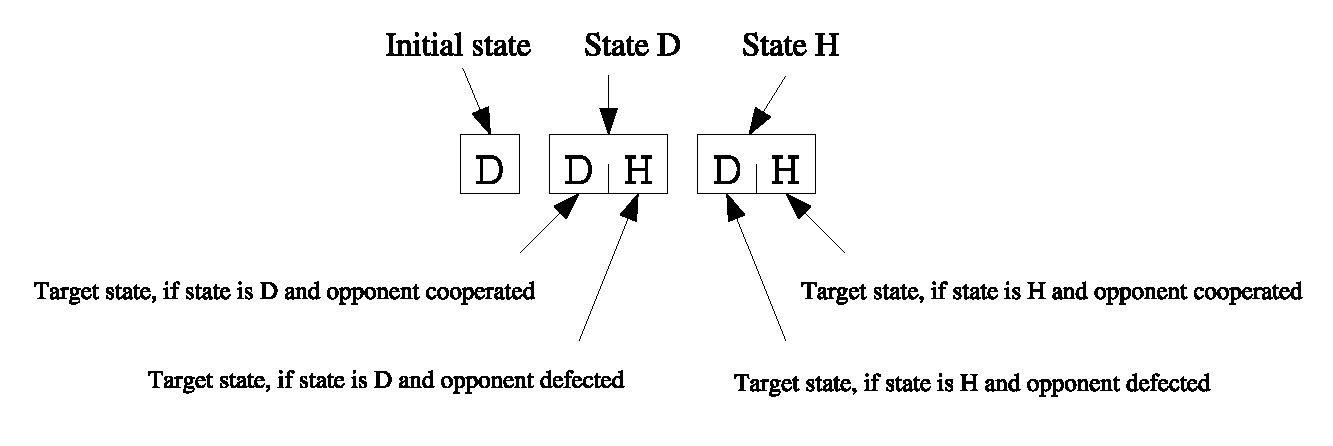
\includegraphics[width=12cm]{images/AutomataRepresentation.eps}
\caption{\label{AutomataRepresentation} Coding players in the repeated
  Prisoner's Dilemma as two state automata. The example shows the
  string representation for the automaton that plays {\em Tit for
    Tat}.}
\end{center}
\end{figure}

Accordingly, two state automata can be implemented by a simple table look-up
algorithm, as can be seen in the following abbreviated code snippet:

\begin{scriptsize}
\begin{verbatim}

class TwoStateAutomaton(Strategy):

    def __init__(self, programString="DDHDH"):
        Strategy.__init__(self)
        self.name = "AM: " + programString

        dic = { 'D':1, 'H':0 }
        self.initialState = dic[programString[0]]
        self.state = self.initialState
        self.progString = programString
        self.prog = [ [dic[programString[4]], dic[programString[3]]], \
                      [dic[programString[2]], dic[programString[1]]] ]

    def firstMove(self):
        self.state = self.initialState
        return self.state

    def nextMove(self, myMoves, opMoves):
        self.state = self.prog[self.state][opMoves[-1]]
        return self.state

\end{verbatim}
\end{scriptsize}

The string representation allows for 32 ($2^5$) different encodings,
but in fact there exist only 26 different automata, because the
automata that represent the strategies {\em Dove} and {\em Hawk} can
be encoded in four different ways (since there are four ($2^2$)
different codings for the state that is never reached). By convenience
we will pick the string representation ``DDDDD'' for the strategy
{\em Dove} and ``HHHHH'' for the strategy {\em Hawk}. Table
\ref{AllTwoStateAutomata} shows all possible two state automata. Some
of them have been given names either to indicate which algorithmic
strategy they represent or just fancy names that where partly taken from
\cite[p. 296]{binmore:1998} (who in turn borrowed them from ``Alice in
Wonderland'').

\begin{figure}
\begin{center}
\begin{tabular}{llll}
1.  & DDDDD (Dove)        & 14. & HDDDD \\
2.  & DDHDD (Tweedledee)  & 15. & HDDDH \\
3.  & DDHDH (Tit for Tat) & 16. & HDDHD (Tweetypie) \\
4.  & DDHHD (Tweedledum)  & 17. & HDHDD (Simpleton) \\
5.  & DDHHH (Grim)        & 18. & HDHDH \\
6.  & DHDDD               & 19. & HDHHD (Pavlov) \\
7.  & DHDDH               & 20. & HHDDD \\
8.  & DHDHD               & 21. & HHDDH \\
9.  & DHDHH               & 22. & HHDHD (Inverted TFT) \\
10. & DHHDD               & 23. & HHHDD \\
11. & DHHDH               & 24. & HHHDH \\
12. & DHHHD               & 25. & HHHHD \\
13. & DHHHH               & 26. & HHHHH \\
\end{tabular}
\caption{\label{AllTwoStateAutomata} List of all possible two state
  automata. The additional names are mostly taken from
  \cite[p. 296]{binmore:1998}.}
\end{center}
\end{figure}


\newpage

\subsection{The family of {\em Signaling Cheater} strategies}
\label{signalingCheaters}

A {\em Singalling Cheater}-strategy is a strategy that plays a predefined
sequence of cooperative and defective moves in the first $n$ rounds of the
repeated Prisoner's Dilemma. If
the opponent player starts with exactly the same sequence of moves, {\em
  Signaling Cheater} assumes that it has met another {\em Signaling Cheater}
and cooperates unconditionally for the remaining rounds of the repeated game.
Otherwise {\em Signaling Cheater} defects for the rest of the game. Thus,
{\em Signaling Cheater} is a strategy that is designed to cooperate only with
its own kind (that is other {\em Signaling Cheaters} that use the same
starting sequence as a signal) and not to cooperate with any other strategy.
The {\tt Python} implementation of {\em Signaling Cheater} follows below:

\begin{scriptsize}
\begin{verbatim}
class SignalingCheater(Strategy):
    def __repr__(self):
        return self.__class__.__name__+"("+repr(self.signal)+")"
    def __init__(self, signal=(0,1,1)):
        Strategy.__init__(self)
        self.signal = signal
        for i in self.signal: self.name += str(i)
    def firstMove(self):
        self.pos = 0
        return self.signal[self.pos]
    def nextMove(self, myMoves, opMoves):
        self.pos += 1
        if self.pos < len(self.signal):
            return self.signal[self.pos]
        else:
            if tuple(opMoves[:len(self.signal)]) == self.signal:
                return 1
            else: return 0
\end{verbatim}
\end{scriptsize}


\newpage

\section{Implementation details of the population dynamics}
\label{implementationDetails}

The population dynamical processes at the base of the simulations in
this book are modeled in a very common and straight forward way: At
the center of most simulations is the evolutionary success of certain
strategies in games such as the repeated Prisoner's Dilemma game. We
assume a population of players where each player plays one of the
strategies. (If this seems to abstract, it may help to think of the
strategies as species and of the players as individuals belonging to
the one or the other species, or to think of the strategies as
mutually exclusive social norms and the players as people that chose
which norm they adhere to.) The players that play a certain strategy
thus constitute the population share of this strategy. For the sake of
simplicity an infinitely large population of players is assumed. The
size of the population share of a strategy is expressed as a fraction
of 1. In the beginning the shares are usually divided equal among all
strategies. The evolutionary process is modeled as a sequence of non
overlapping generational cycles. During each generation the fitness of
every strategy is determined by the average score in the tournament,
where the score of each match is weighted with the population share of
the opponent.  Thus the fitness is determined by:

\begin{equation}
\label{fitnessEquation}
F_i = \sum_{k=1}^n S_{ik}P_k
\end{equation}
\begin{tabular}{lll}
  $F_i$    & &  the Fitness of the $i$-th strategy \\
  $S_{ik}$  & & the score of the $i$-th strategy when playing against
the $k$-th strategy \\
  $P_k$  & & the population share of $k$-th strategy \\
  $n$ & & the total number of strategies in the simulation \\
  $i,k$ & & indices of the strategies \\
& & \\
\end{tabular}

In the simulation program the calculation of the fitness is performed by one
of the different {\tt Fitness} functions in module {\tt Dynamics\-.\-py} of
package {\tt Population\-Dynamics}. The simplemost of these is the function
{\tt Dynamics\-.\-\_Quick\-Fitness2}. If calculates the fitness values of a
population of strategies based on a two player game. The function {\tt
  \_QuickFitness2} is called with the tuple of population shares and the
payoff matrix as parameters. The payoff matrix contains the payoff of the
matches of each strategy against every other strategy. The function returns
the list of fitness values of the strategies.\footnote{This and the following
  code snipplets are taken from module {\tt PopulationDynamics.Dynamics}. For
  the sake of brevity and better readability the error checking code has been
  left out here.}

\begin{scriptsize}
\begin{verbatim}
 1: def _QuickFitness2(population, payoff):
 2:     n = population
 3:     L = len(n)
 4:     p = []
 5:     for i in xrange(L):
 6:         s = 0.0
 7:         for k in xrange(L):
 8:             s += payoff[i,k]*n[k]
 9:         p.append(s)
10:     return p
\end{verbatim}
\end{scriptsize}

The fitness $F_i$ of equation \ref{fitnessEquation} is calculated in
the {\tt for} loop in lines 7 and 8. The outer {\tt for} loop (lines 5
to 9) calculates the fitness for each strategy and appends it to the
list of fitness values. (The assignment in line 2 is done just for
convenience to avoid to many long variable names in line 8.)

One of the parameters that is varied in the simulation series' (see
\ref{refinedModel}) is the parameter {\em e} for the correlation of players of
the same strategy. If {\em e} is nonzero then players with the same strategy
interact more often than with purely random matching. In order to integrate
correlation into the model the original fitness equation
(\ref{fitnessEquation}) must be slightly changed.\footnote{This very simple
  model of correlation was taken from \cite[p. 113, note 30]{skyrms:1996}.}

\begin{equation}
\label{extendedFitnessEquation}
F_i = \sum_{\substack{k = 1 \\ k \ne i}}^n S_{ik}(1-e)P_k + S_{ii}(P_i +
e(1-P_i))
\end{equation}
\begin{tabular}{lll}
  $F_i$    & &  the Fitness of the $i$-th strategy \\
  $S_{ik}$  & & the score of the $i$-th strategy when playing against
the $k$-th strategy \\
  $P_k$  & & the population share of $k$-th strategy \\
  $n$ & & the total number of strategies in the simulation \\
  $i,k$ & & indices of the strategies \\
  $e$ & & the correlation factor, ranging from 0 to 1 \\
& & \\
\end{tabular}

It should be observed that if the correlation $e=0$ then equation
(\ref{extendedFitnessEquation} resolves to the simpler equation
(\ref{fitnessEquation}). But if the correlation $e=1$ (perfect correlation)
then $F_i = S_{ii}$, which is exactly what we would expect: When the
correlation is perfect, players of one strategy never interact with players
of any other strategy and their fitness depends entirely on how the strategy
scores against itself. The implementation of the fitness functions that
includes correlation looks accordingly:

\begin{scriptsize}
\begin{verbatim}
 1: def _Fitness2(population, payoff, e):
 2:     n = population
 3:     L = len(n) 
 4:     p = []    
 5:     for i in xrange(L):
 6:         s = 0.0
 7:         for k in xrange(L):
 8:             if i == k:
 9:                 s += payoff[i,k]*(n[i]+e*(1.0-n[i]))
10:             else: 
11:                 s += payoff[i,k]*(n[k]-e*n[k])
12:         p.append(s)
13:     return p
\end{verbatim}
\end{scriptsize}

The population shares of the next generation are then determined simply by
multiplying the population share of each strategy with its fitness. Since we
calculate with population shares and not with absolute population sizes the
fitness values always express relative fitness. (It makes no difference if
strategy A has a fitness of 1 and strategy B has a fitness of 2 or if A has
fitness 50 and B fitness 100.)  For convenience, the population shares are
normalized (by dividing them through the sum of the not normalized population
shares) so that they nicely add up to 1:

\begin{equation}
\label{populationEquation}
P_i^{g+1} = \frac{P_i^gF_i^g}{\sum_{k=1}^n P_k^gF_k^g}
\end{equation}
\begin{tabular}{lll}
$P_i^g$ & & the population share of strategy $i$ in generation $g$ \\
$F_i^g$ & & the fitness of the $i$-th strategy in generation $g$ \\
$g$ & & the number of the current generation \\
$i,k$ & & indices of the strategies \\
& & \\
\end{tabular} 

The program code that performs these calculations looks as follows:

\begin{scriptsize}
\begin{verbatim}
 1: def _QuickReplicator(population, fitness):
 2:     n = list(population)
 3:     L = len(population)
 4:     f = fitness(population)
 5:     for i in xrange(L): n[i] *= f[i]
 6:     N = sum(n)
 7:     for i in xrange(L): n[i] /= N
 8:     return tuple(n)
\end{verbatim}
\end{scriptsize}

The function {\tt Dynamics\-.\-\_Quick\-Replicator} of package {\tt
  Population\-Dynamics} takes the tuple of population shares and a
fitness function as parameters and returns the tuple of population
shares of the next generation. The fitness function is called in line
4. It is expected to return a list with the fitness values of the
strategies. (As it takes only one parameter the above fitness
function, which takes two parameters, cannot be called directly from
the replicator function, but must be called indirectly through a
dynamically created function that includes the payoff matrix as a
constant parameter. There are technical reasons for using this
construction instead of passing through the payoff matrix from the
caller of the replicator function to the fitness function.) The actual
calculation of the next generation's population shares $P_i^{g+1}$ of
equation \ref{populationEquation} are carried out in lines 5 to 8.

Just as in the case of the fitness equation (\ref{fitnessEquation}) and the
related program code there exists an extended version of the population
equation (\ref{populationEquation}) for the case when the background noise $b
> 0$: 

\begin{equation}
\label{extendedPopulationEquation}
P_i^{g+1} = \frac{P_i^gF_i^g(1-bR_i^g)}{\sum_{k=1}^n P_k^gF_k^g(1-bR_k^g)}
\end{equation}
\begin{tabular}{lll}
$P_i^g$ & & the population share of strategy $i$ in generation $g$ \\
$F_i$ & & the fitness of the $i$-th strategy in generation $g$ \\
$g$ & & the number of the current generation \\
$i,k$ & & indices of the strategies \\
$b$ & & evolutionary background noise $ 0 \le b \le 1$ \\
$R_i^g$ & & a random number $0 \le R_i^g < 1$ \\
& & \\
\end{tabular} 

The implementation in {\tt Python} code is likewise:

\begin{scriptsize}
\begin{verbatim}
 1: def _Replicator(population, fitness, noise):
 2:     n = list(population)
 3:     L = len(population)
 4:     f = fitness
 5:     for i in xrange(L):  n[i] *= f[i]- random.uniform(0,f[i]*noise)
 6:     N = sum(n)
 7:     for i in xrange(L): n[i] /= N
 8:     return tuple(n)
\end{verbatim}
\end{scriptsize}

A few things need to be noted about the model as well as its implementation.
When using infinite populations this is of course an idealization. It makes it
easier to calculate with population shares and, as the model is purely
conceptual and we do not have any particular empirical application of the
model in mind, any fixed finite population size would be arbitrary anyway.
However, the use of infinite populations for modeling processes that take
place in finite populations slightly distorts the evolutionary process in two
ways: 1) Even the slightest variations in fitness lead to variations in
population shares.  In real life, or in nature for that matter, it is
conceivable that very small fitness differences are not strong enough to
transform into a different number of offspring\footnote{It is important here
  that the fitness and the number of offspring are not the same by definition.
  For a short discussion of this point see page \pageref{tautologyCharge}.}
and 2) and more importantly, as long as the fitness value remains above zero,
a species (or strategy respectively) can never die out. Its population share
could be arbitrarily small, yet there is still a possibility that it will
eventually recover, even though in ``real life'' it would never be given a
second chance.  Of course, both of these distortions can, if necessary, easily
be remedied by 1) mapping the fitness onto a discrete set of numbers before
calculating the population shares of the next generation and 2) defining a
threshold population share below which a species (or strategy in our case)
will be eliminated from the population, but it is important to keep these
points in mind.

They way in which the fitness is derived from the payoffs in the
(Prisoner's Dilemma) game also introduces certain peculiarities.
Because the weighted average payoff is used as fitness value, negative
payoffs are impermissible. This may seem awkward given that negative
payoffs are usually perfectly legitimate in game theory and might even
be given a reasonable interpretation, for example, to indicate a loss
of money in an economical context. But if we think of fitness in an
evolutionary context, it makes perfectly good sense to exclude negative
payoffs, because the reproduction rate cannot conceivably fall below
zero. A reproduction rate of zero already means -- depending on the
context -- the extinction of a species, the vanishing of a gene or the
disappearance of a social norm. What worse could happen in evolution
than extinction?

The simulation models described in sections \ref{simpleModel} and
\ref{refinedModel} do even make it impossible that the fitness value
will be exactly zero, because even though some strategies may be left
with a payoff of zero in the repeated Prisoner's Dilemma match against
another strategy (as, for example, {\em Dove} against {\em Hawk}) the
average payoff of a strategy in the tournament can never be zero,
because no strategy gets a zero payoff in the match against itself.
This simplifies calculations greatly, because no provisions for the
special case of a zero fitness need to be made. Otherwise, care would
have to be taken to avoid divisions by zero and the like.

\newpage
\section{Comprehensive results of the simualtion series}
\label{completeTables}

The following tables and figures list all of aggregated data of the simulation
series described in chapter \ref{refinedModel}. First (section
\ref{BigSeriesResults}) the overall results of the big series are given, both
as tables and then in a graphical form. The stratgey set of {\em Two State
Automata} (section \ref{twoStateAutomata} above) and the set of {\em
Parameterized Tit for Tats} (section \ref{parameterizedTFTs}) are always
considered separately. In the tables the the average final population shares
of the evolutionary simulations is displayed. (The simulations in the series
were stopped either when no changes in the composition of the population
occured any more or when the 25,600th generation had been reached.) The
strategies are always ranked after their average final population share in the
whole series. The graphical representation depicts in three columns the
tournament ranking (in lexical order that is, if a strategy has been the the
winner of the tournament two times over the whole series it is always better
than a strategy that has won the tournament only once, no matter how often it
was placed second), the evolutionary ranking (by the average final population
share) and a more illustrative representation of the evolutionary ranking. On
the graphical representation, the strategies are represented by colored bars,
which represent their degree of altruism. A green color means that the strategy
is fully (e.g. {\em Dove}) or to some degree (e.g. {\em Tweedledee}) genuinely
altruistic. A blue color means that it is either reciprocal (e.g. {\em Tit for
Tat}, {\em Grim}) or cannot be classified (e.g. {\em Inverted}). Red means that
the strategy is a cheater or (primarily) non altruistic (e.g. {\em Hawk}). (See
page \pageref{colorScheme} for detailed description of the color scheme and its
motivation.)

In order to determine the influence of single parameters on the simulation, the
aggregated results for every parameter held constant at each of its values (see
page \pageref{seriesParameters}) was calculated as well. This helps to
find out about the influence of single parameters on the simulation, though
possible joint effects of several parameters still remain opaque. For each
parameter and strategy set, a table is presented that shows how the average
final population share of each strategy changes for different values of the
parameter. There is also a graphical representation of the tournament rankings
and evolutionary outcomes for each parameter value and strategy set.

\newpage
\subsection{``Big series'' overall results}
\label{BigSeriesResults}

\begin{tabular}{|l|r|}
\hline
 & \multicolumn{1}{c|}{{\bf Average Final Population Share}} \\
\hline
{\bf Strategy} & overall results\\ \hline
AM: HHHHH (HAWK)             &   34.61 \% \\
AM: DDHHH (GRIM)             &   17.28 \% \\
AM: DDHDH (TIT FOR TAT)      &   10.22 \% \\
AM: HDHHD (PAVLOV)           &   10.01 \% \\
AM: DDDDD (DOVE)             &    9.27 \% \\
AM: DDHHD (TWEEDLEDUM)       &    7.12 \% \\
AM: DDHDD (TWEEDLEDEE)       &    2.91 \% \\
AM: HDHDH (TAT FOR TIT)      &    1.73 \% \\
AM: DHHHH                    &    1.56 \% \\
AM: DHHDH                    &    1.39 \% \\
AM: HDHDD (SIMPLETON)        &    1.28 \% \\
AM: HHHDH                    &    1.09 \% \\
AM: HHHHD                    &    0.52 \% \\
AM: DHHDD                    &    0.39 \% \\
AM: HHHDD                    &    0.36 \% \\
AM: DHHHD                    &    0.13 \% \\
AM: DHDHH                    &    0.10 \% \\
AM: HDDHD (TWEETYPIE)        &    0.00 \% \\
AM: HHDHD (INVERTED)         &    0.00 \% \\
AM: DHDHD                    &    0.00 \% \\
AM: HDDDD                    &    0.00 \% \\
AM: HHDDD                    &    0.00 \% \\
AM: DHDDD                    &    0.00 \% \\
AM: HDDDH                    &    0.00 \% \\
AM: HHDDH                    &    0.00 \% \\
AM: DHDDH                    &    0.00 \% \\
\hline
\end{tabular}


\newpage
\begin{tabular}{|l|r|}
\hline
 & \multicolumn{1}{c|}{{\bf Average Final Population Share}} \\
\hline
{\bf Strategy} & overall results\\ \hline
P\_TFT 0.00 0.00 (TitForTat)  &   38.54 \% \\
P\_TFT 0.00 1.00 (Hawk)       &   28.50 \% \\
P\_TFT 0.20 0.00              &    8.98 \% \\
P\_TFT 1.00 0.00 (Dove)       &    8.30 \% \\
P\_TFT 0.40 0.00              &    8.27 \% \\
P\_TFT 0.80 0.00              &    2.16 \% \\
P\_TFT 1.00 1.00 (Inverted)   &    1.55 \% \\
P\_TFT 0.00 0.80              &    1.06 \% \\
P\_TFT 0.20 0.40              &    0.93 \% \\
P\_TFT 0.60 0.00              &    0.51 \% \\
P\_TFT 0.40 0.20              &    0.46 \% \\
P\_TFT 0.60 1.00              &    0.38 \% \\
P\_TFT 0.40 0.40              &    0.23 \% \\
P\_TFT 0.60 0.20              &    0.12 \% \\
P\_TFT 0.80 1.00              &    0.01 \% \\
P\_TFT 0.40 1.00              &    0.00 \% \\
P\_TFT 0.20 1.00              &    0.00 \% \\
P\_TFT 0.00 0.60              &    0.00 \% \\
P\_TFT 0.80 0.20              &    0.00 \% \\
P\_TFT 1.00 0.20              &    0.00 \% \\
P\_TFT 0.80 0.40              &    0.00 \% \\
P\_TFT 0.20 0.20              &    0.00 \% \\
P\_TFT 0.60 0.40              &    0.00 \% \\
P\_TFT 1.00 0.40              &    0.00 \% \\
P\_TFT 0.00 0.40              &    0.00 \% \\
P\_TFT 0.80 0.60              &    0.00 \% \\
P\_TFT 1.00 0.60              &    0.00 \% \\
P\_TFT 0.00 0.20              &    0.00 \% \\
P\_TFT 0.60 0.60              &    0.00 \% \\
P\_TFT 0.40 0.60              &    0.00 \% \\
P\_TFT 0.20 0.60              &    0.00 \% \\
P\_TFT 0.80 0.80              &    0.00 \% \\
P\_TFT 0.20 0.80              &    0.00 \% \\
P\_TFT 0.60 0.80              &    0.00 \% \\
P\_TFT 0.40 0.80              &    0.00 \% \\
P\_TFT 1.00 0.80              &    0.00 \% \\
\hline
\end{tabular}


\begin{sidewaysfigure}
\begin{center}
\includegraphics[width=20cm]{tables/Automata_overall.eps}
\caption{\label{Automata_Overall} The aggregated results of all simulations
of the ``big series'' using {\em Automata} strategies.}
\end{center}
\end{sidewaysfigure}

\begin{sidewaysfigure}
\begin{center}
\includegraphics[width=20cm]{tables/TFTs_overall.eps}
\caption{\label{TFTs_Overall} The aggregated results of all simulations
of the ``big series'' using {\em Parameterized Tit for Tat} strategies.}
\end{center}
\end{sidewaysfigure}


\newpage
\subsection{The influence of correlation}

The correlation factor describes the probability by which players are
more likely to meet opponents with the same strategy than opponents with a
different strategy. A correlation of 0\% means that the players are randomly
matched, while with a correlation of 100\% players do exclusively play
against players of the same strategy.

\subsubsection{Automata}
\begin{tabular}{|l|r|r|r|r|}
\hline
 & \multicolumn{4}{c|}{{\bf Average Final Population Share}} \\
\hline
{\bf Strategy} & overall &  c = 0.0 & c = 0.1 & c = 0.2\\ \hline
AM: HHHHH (HAWK)             &   34.61 \%  &   44.30 \%  &   33.71 \%  &   25.81 \% \\
AM: DDHHH (GRIM)             &   17.28 \%  &   21.73 \%  &   16.27 \%  &   13.85 \% \\
AM: DDHDH (TIT FOR TAT)      &   10.22 \%  &    9.51 \%  &   13.47 \%  &    7.69 \% \\
AM: HDHHD (PAVLOV)           &   10.01 \%  &    2.08 \%  &    4.83 \%  &   23.11 \% \\
AM: DDDDD (DOVE)             &    9.27 \%  &    8.04 \%  &   11.29 \%  &    8.48 \% \\
AM: DDHHD (TWEEDLEDUM)       &    7.12 \%  &    2.58 \%  &    4.95 \%  &   13.82 \% \\
AM: DDHDD (TWEEDLEDEE)       &    2.91 \%  &    2.70 \%  &    4.40 \%  &    1.63 \% \\
AM: HDHDH (TAT FOR TIT)      &    1.73 \%  &    0.00 \%  &    1.88 \%  &    3.32 \% \\
AM: DHHHH                    &    1.56 \%  &    4.69 \%  &    0.00 \%  &    0.00 \% \\
AM: DHHDH                    &    1.39 \%  &    0.53 \%  &    2.62 \%  &    1.02 \% \\
AM: HDHDD (SIMPLETON)        &    1.28 \%  &    0.62 \%  &    2.57 \%  &    0.66 \% \\
AM: HHHDH                    &    1.09 \%  &    0.56 \%  &    2.11 \%  &    0.61 \% \\
AM: HHHHD                    &    0.52 \%  &    0.78 \%  &    0.79 \%  &    0.00 \% \\
AM: DHHDD                    &    0.39 \%  &    0.86 \%  &    0.32 \%  &    0.00 \% \\
AM: HHHDD                    &    0.36 \%  &    0.70 \%  &    0.39 \%  &    0.00 \% \\
AM: DHHHD                    &    0.13 \%  &    0.00 \%  &    0.40 \%  &    0.00 \% \\
AM: DHDHH                    &    0.10 \%  &    0.29 \%  &    0.00 \%  &    0.00 \% \\
AM: HDDHD (TWEETYPIE)        &    0.00 \%  &    0.00 \%  &    0.00 \%  &    0.00 \% \\
AM: HHDHD (INVERTED)         &    0.00 \%  &    0.00 \%  &    0.00 \%  &    0.00 \% \\
AM: DHDHD                    &    0.00 \%  &    0.00 \%  &    0.00 \%  &    0.00 \% \\
AM: HDDDD                    &    0.00 \%  &    0.00 \%  &    0.00 \%  &    0.00 \% \\
AM: HHDDD                    &    0.00 \%  &    0.00 \%  &    0.00 \%  &    0.00 \% \\
AM: DHDDD                    &    0.00 \%  &    0.00 \%  &    0.00 \%  &    0.00 \% \\
AM: HDDDH                    &    0.00 \%  &    0.00 \%  &    0.00 \%  &    0.00 \% \\
AM: HHDDH                    &    0.00 \%  &    0.00 \%  &    0.00 \%  &    0.00 \% \\
AM: DHDDH                    &    0.00 \%  &    0.00 \%  &    0.00 \%  &    0.00 \% \\
\hline
\end{tabular}


\begin{sidewaysfigure}
\begin{center}
\includegraphics[width=20cm]{tables/Automata_C0.000.eps}
\caption{\label{Automata_C0000} The aggregated results of those
simulations of the ``big series'' for which the correlation value was 0\%.}
\end{center}
\end{sidewaysfigure}

\begin{sidewaysfigure}
\begin{center}
\includegraphics[width=20cm]{tables/Automata_C0.100.eps}
\caption{\label{Automata_C0100} The aggregated results of those
simulations of the ``big series'' for which the correlation value was 10\%.}
\end{center}
\end{sidewaysfigure}

\begin{sidewaysfigure}
\begin{center}
\includegraphics[width=20cm]{tables/Automata_C0.200.eps}
\caption{\label{Automata_C0200} The aggregated results of those
simulations of the ``big series'' for which the correlation value was 20\%.}
\end{center}
\end{sidewaysfigure}

\newpage
\subsubsection{Parameterized Tit for Tats}
\begin{tabular}{|l|r|r|r|r|}
\hline
 & \multicolumn{4}{c|}{{\bf Average Final Population Share}} \\
\hline
{\bf Strategy} & overall &  c = 0.0 & c = 0.1 & c = 0.2\\ \hline
P\_TFT 0.00 0.00 (TitForTat)  &   38.54 \%  &   32.71 \%  &   42.20 \%  &   40.72 \% \\
P\_TFT 0.00 1.00 (Hawk)       &   28.50 \%  &   54.45 \%  &   25.76 \%  &    5.29 \% \\
P\_TFT 0.20 0.00              &    8.98 \%  &    0.87 \%  &    6.84 \%  &   19.22 \% \\
P\_TFT 1.00 0.00 (Dove)       &    8.30 \%  &    1.27 \%  &    7.15 \%  &   16.49 \% \\
P\_TFT 0.40 0.00              &    8.27 \%  &    4.14 \%  &    9.60 \%  &   11.06 \% \\
P\_TFT 0.80 0.00              &    2.16 \%  &    0.70 \%  &    2.11 \%  &    3.68 \% \\
P\_TFT 1.00 1.00 (Inverted)   &    1.55 \%  &    1.24 \%  &    1.54 \%  &    1.88 \% \\
P\_TFT 0.00 0.80              &    1.06 \%  &    1.80 \%  &    1.37 \%  &    0.00 \% \\
P\_TFT 0.20 0.40              &    0.93 \%  &    2.78 \%  &    0.00 \%  &    0.00 \% \\
P\_TFT 0.60 0.00              &    0.51 \%  &    0.05 \%  &    0.78 \%  &    0.70 \% \\
P\_TFT 0.40 0.20              &    0.46 \%  &    0.00 \%  &    1.39 \%  &    0.00 \% \\
P\_TFT 0.60 1.00              &    0.38 \%  &    0.00 \%  &    0.37 \%  &    0.78 \% \\
P\_TFT 0.40 0.40              &    0.23 \%  &    0.00 \%  &    0.69 \%  &    0.00 \% \\
P\_TFT 0.60 0.20              &    0.12 \%  &    0.00 \%  &    0.19 \%  &    0.17 \% \\
P\_TFT 0.80 1.00              &    0.01 \%  &    0.00 \%  &    0.02 \%  &    0.01 \% \\
P\_TFT 0.40 1.00              &    0.00 \%  &    0.00 \%  &    0.00 \%  &    0.00 \% \\
P\_TFT 0.20 1.00              &    0.00 \%  &    0.00 \%  &    0.00 \%  &    0.00 \% \\
P\_TFT 0.00 0.60              &    0.00 \%  &    0.00 \%  &    0.00 \%  &    0.00 \% \\
P\_TFT 0.80 0.20              &    0.00 \%  &    0.00 \%  &    0.00 \%  &    0.00 \% \\
P\_TFT 1.00 0.20              &    0.00 \%  &    0.00 \%  &    0.00 \%  &    0.00 \% \\
P\_TFT 0.80 0.40              &    0.00 \%  &    0.00 \%  &    0.00 \%  &    0.00 \% \\
P\_TFT 0.20 0.20              &    0.00 \%  &    0.00 \%  &    0.00 \%  &    0.00 \% \\
P\_TFT 0.60 0.40              &    0.00 \%  &    0.00 \%  &    0.00 \%  &    0.00 \% \\
P\_TFT 1.00 0.40              &    0.00 \%  &    0.00 \%  &    0.00 \%  &    0.00 \% \\
P\_TFT 0.00 0.40              &    0.00 \%  &    0.00 \%  &    0.00 \%  &    0.00 \% \\
P\_TFT 0.80 0.60              &    0.00 \%  &    0.00 \%  &    0.00 \%  &    0.00 \% \\
P\_TFT 1.00 0.60              &    0.00 \%  &    0.00 \%  &    0.00 \%  &    0.00 \% \\
P\_TFT 0.00 0.20              &    0.00 \%  &    0.00 \%  &    0.00 \%  &    0.00 \% \\
P\_TFT 0.60 0.60              &    0.00 \%  &    0.00 \%  &    0.00 \%  &    0.00 \% \\
P\_TFT 0.40 0.60              &    0.00 \%  &    0.00 \%  &    0.00 \%  &    0.00 \% \\
P\_TFT 0.20 0.60              &    0.00 \%  &    0.00 \%  &    0.00 \%  &    0.00 \% \\
P\_TFT 0.80 0.80              &    0.00 \%  &    0.00 \%  &    0.00 \%  &    0.00 \% \\
P\_TFT 0.20 0.80              &    0.00 \%  &    0.00 \%  &    0.00 \%  &    0.00 \% \\
P\_TFT 0.60 0.80              &    0.00 \%  &    0.00 \%  &    0.00 \%  &    0.00 \% \\
P\_TFT 0.40 0.80              &    0.00 \%  &    0.00 \%  &    0.00 \%  &    0.00 \% \\
P\_TFT 1.00 0.80              &    0.00 \%  &    0.00 \%  &    0.00 \%  &    0.00 \% \\
\hline
\end{tabular}


\begin{sidewaysfigure}
\begin{center}
\includegraphics[width=20cm]{tables/TFTs_C0.000.eps}
\caption{\label{TFTs_C0000} The aggregated results of those
simulations of the ``big series'' for which the correlation value was 0\%.}
\end{center}
\end{sidewaysfigure}

\begin{sidewaysfigure}
\begin{center}
\includegraphics[width=20cm]{tables/TFTs_C0.100.eps}
\caption{\label{TFTs_C0100} The aggregated results of those
simulations of the ``big series'' for which the correlation value was 10\%.}
\end{center}
\end{sidewaysfigure}

\begin{sidewaysfigure}
\begin{center}
\includegraphics[width=20cm]{tables/TFTs_C0.200.eps}
\caption{\label{TFTs_C0200} The aggregated results of those
simulations of the ``big series'' for which the correlation value was 20\%.}
\end{center}
\end{sidewaysfigure}


\newpage
\subsection{The influence of game noise}

The game noise parameter specifies a probability with which the
intended move of a player is randomly turned into its opposite.

\subsubsection{Automata}
\begin{tabular}{|l|r|r|r|r|}
\hline
 & \multicolumn{4}{c|}{{\bf Average Final Population Share}} \\
\hline
{\bf Strategy} & overall &  g = 0.0 & g = 0.05 & g = 0.1\\ \hline
AM: HHHHH (HAWK)             &   34.61 \%  &    7.45 \%  &   36.38 \%  &   59.99 \% \\
AM: DDHHH (GRIM)             &   17.28 \%  &   38.23 \%  &   10.42 \%  &    3.19 \% \\
AM: DDHDH (TIT FOR TAT)      &   10.22 \%  &   15.82 \%  &    7.78 \%  &    7.07 \% \\
AM: HDHHD (PAVLOV)           &   10.01 \%  &    5.03 \%  &   16.48 \%  &    8.51 \% \\
AM: DDDDD (DOVE)             &    9.27 \%  &   22.58 \%  &    3.67 \%  &    1.56 \% \\
AM: DDHHD (TWEEDLEDUM)       &    7.12 \%  &    7.08 \%  &    9.13 \%  &    5.14 \% \\
AM: DDHDD (TWEEDLEDEE)       &    2.91 \%  &    3.81 \%  &    4.66 \%  &    0.26 \% \\
AM: HDHDH (TAT FOR TIT)      &    1.73 \%  &    0.00 \%  &    2.57 \%  &    2.64 \% \\
AM: DHHHH                    &    1.56 \%  &    0.00 \%  &    0.74 \%  &    3.95 \% \\
AM: DHHDH                    &    1.39 \%  &    0.00 \%  &    1.72 \%  &    2.45 \% \\
AM: HDHDD (SIMPLETON)        &    1.28 \%  &    0.00 \%  &    0.93 \%  &    2.92 \% \\
AM: HHHDH                    &    1.09 \%  &    0.00 \%  &    2.02 \%  &    1.26 \% \\
AM: HHHHD                    &    0.52 \%  &    0.00 \%  &    1.46 \%  &    0.12 \% \\
AM: DHHDD                    &    0.39 \%  &    0.00 \%  &    1.01 \%  &    0.17 \% \\
AM: HHHDD                    &    0.36 \%  &    0.00 \%  &    0.86 \%  &    0.23 \% \\
AM: DHHHD                    &    0.13 \%  &    0.00 \%  &    0.16 \%  &    0.24 \% \\
AM: DHDHH                    &    0.10 \%  &    0.00 \%  &    0.00 \%  &    0.29 \% \\
AM: HDDHD (TWEETYPIE)        &    0.00 \%  &    0.00 \%  &    0.00 \%  &    0.00 \% \\
AM: HHDHD (INVERTED)         &    0.00 \%  &    0.00 \%  &    0.00 \%  &    0.00 \% \\
AM: DHDHD                    &    0.00 \%  &    0.00 \%  &    0.00 \%  &    0.00 \% \\
AM: HDDDD                    &    0.00 \%  &    0.00 \%  &    0.00 \%  &    0.00 \% \\
AM: HHDDD                    &    0.00 \%  &    0.00 \%  &    0.00 \%  &    0.00 \% \\
AM: DHDDD                    &    0.00 \%  &    0.00 \%  &    0.00 \%  &    0.00 \% \\
AM: HDDDH                    &    0.00 \%  &    0.00 \%  &    0.00 \%  &    0.00 \% \\
AM: HHDDH                    &    0.00 \%  &    0.00 \%  &    0.00 \%  &    0.00 \% \\
AM: DHDDH                    &    0.00 \%  &    0.00 \%  &    0.00 \%  &    0.00 \% \\
\hline
\end{tabular}


\begin{sidewaysfigure}
\begin{center}
\includegraphics[width=20cm]{tables/Automata_G0.000.eps}
\caption{\label{Automata_G0000} The aggregated results of those
simulations of the ``big series'' for which the game noise was 0\%.}
\end{center}
\end{sidewaysfigure}

\begin{sidewaysfigure}
\begin{center}
\includegraphics[width=20cm]{tables/Automata_G0.050.eps}
\caption{\label{Automata_G0050} The aggregated results of those
simulations of the ``big series'' for which the game noise was 5\%.}
\end{center}
\end{sidewaysfigure}

\begin{sidewaysfigure}
\begin{center}
\includegraphics[width=20cm]{tables/Automata_G0.100.eps}
\caption{\label{Automata_G0100} The aggregated results of those
simulations of the ``big series'' for which the game noise was 10\%.}
\end{center}
\end{sidewaysfigure}

\newpage
\subsubsection{Parameterized Tit for Tats}
\begin{tabular}{|l|r|r|r|r|}
\hline
 & \multicolumn{4}{c|}{{\bf Average Final Population Share}} \\
\hline
{\bf Strategy} & overall &  g = 0.0 & g = 0.05 & g = 0.1\\ \hline
P\_TFT 0.00 0.00 (TitForTat)  &   38.54 \%  &   82.41 \%  &   18.98 \%  &   14.24 \% \\
P\_TFT 0.00 1.00 (Hawk)       &   28.50 \%  &    0.00 \%  &   27.39 \%  &   58.11 \% \\
P\_TFT 0.20 0.00              &    8.98 \%  &    6.84 \%  &    8.60 \%  &   11.48 \% \\
P\_TFT 1.00 0.00 (Dove)       &    8.30 \%  &    6.56 \%  &   11.80 \%  &    6.56 \% \\
P\_TFT 0.40 0.00              &    8.27 \%  &    2.60 \%  &   18.94 \%  &    3.25 \% \\
P\_TFT 0.80 0.00              &    2.16 \%  &    0.93 \%  &    4.17 \%  &    1.39 \% \\
P\_TFT 1.00 1.00 (Inverted)   &    1.55 \%  &    0.00 \%  &    3.00 \%  &    1.66 \% \\
P\_TFT 0.00 0.80              &    1.06 \%  &    0.00 \%  &    3.17 \%  &    0.00 \% \\
P\_TFT 0.20 0.40              &    0.93 \%  &    0.00 \%  &    2.78 \%  &    0.00 \% \\
P\_TFT 0.60 0.00              &    0.51 \%  &    0.65 \%  &    0.00 \%  &    0.87 \% \\
P\_TFT 0.40 0.20              &    0.46 \%  &    0.00 \%  &    0.00 \%  &    1.39 \% \\
P\_TFT 0.60 1.00              &    0.38 \%  &    0.00 \%  &    0.13 \%  &    1.02 \% \\
P\_TFT 0.40 0.40              &    0.23 \%  &    0.00 \%  &    0.69 \%  &    0.00 \% \\
P\_TFT 0.60 0.20              &    0.12 \%  &    0.00 \%  &    0.36 \%  &    0.00 \% \\
P\_TFT 0.80 1.00              &    0.01 \%  &    0.00 \%  &    0.00 \%  &    0.03 \% \\
P\_TFT 0.40 1.00              &    0.00 \%  &    0.00 \%  &    0.00 \%  &    0.00 \% \\
P\_TFT 0.20 1.00              &    0.00 \%  &    0.00 \%  &    0.00 \%  &    0.00 \% \\
P\_TFT 0.00 0.60              &    0.00 \%  &    0.00 \%  &    0.00 \%  &    0.00 \% \\
P\_TFT 0.80 0.20              &    0.00 \%  &    0.00 \%  &    0.00 \%  &    0.00 \% \\
P\_TFT 1.00 0.20              &    0.00 \%  &    0.00 \%  &    0.00 \%  &    0.00 \% \\
P\_TFT 0.80 0.40              &    0.00 \%  &    0.00 \%  &    0.00 \%  &    0.00 \% \\
P\_TFT 0.20 0.20              &    0.00 \%  &    0.00 \%  &    0.00 \%  &    0.00 \% \\
P\_TFT 0.60 0.40              &    0.00 \%  &    0.00 \%  &    0.00 \%  &    0.00 \% \\
P\_TFT 1.00 0.40              &    0.00 \%  &    0.00 \%  &    0.00 \%  &    0.00 \% \\
P\_TFT 0.00 0.40              &    0.00 \%  &    0.00 \%  &    0.00 \%  &    0.00 \% \\
P\_TFT 0.80 0.60              &    0.00 \%  &    0.00 \%  &    0.00 \%  &    0.00 \% \\
P\_TFT 1.00 0.60              &    0.00 \%  &    0.00 \%  &    0.00 \%  &    0.00 \% \\
P\_TFT 0.00 0.20              &    0.00 \%  &    0.00 \%  &    0.00 \%  &    0.00 \% \\
P\_TFT 0.60 0.60              &    0.00 \%  &    0.00 \%  &    0.00 \%  &    0.00 \% \\
P\_TFT 0.40 0.60              &    0.00 \%  &    0.00 \%  &    0.00 \%  &    0.00 \% \\
P\_TFT 0.20 0.60              &    0.00 \%  &    0.00 \%  &    0.00 \%  &    0.00 \% \\
P\_TFT 0.80 0.80              &    0.00 \%  &    0.00 \%  &    0.00 \%  &    0.00 \% \\
P\_TFT 0.20 0.80              &    0.00 \%  &    0.00 \%  &    0.00 \%  &    0.00 \% \\
P\_TFT 0.60 0.80              &    0.00 \%  &    0.00 \%  &    0.00 \%  &    0.00 \% \\
P\_TFT 0.40 0.80              &    0.00 \%  &    0.00 \%  &    0.00 \%  &    0.00 \% \\
P\_TFT 1.00 0.80              &    0.00 \%  &    0.00 \%  &    0.00 \%  &    0.00 \% \\
\hline
\end{tabular}


\begin{sidewaysfigure}
\begin{center}
\includegraphics[width=20cm]{tables/TFTs_G0.000.eps}
\caption{\label{TFTs_G0000} The aggregated results of those
simulations of the ``big series'' for which the game noise was 0\%.}
\end{center}
\end{sidewaysfigure}

\begin{sidewaysfigure}
\begin{center}
\includegraphics[width=20cm]{tables/TFTs_G0.050.eps}
\caption{\label{TFTs_G0050} The aggregated results of those
simulations of the ``big series'' for which the game noise was 5\%.}
\end{center}
\end{sidewaysfigure}

\begin{sidewaysfigure}
\begin{center}
\includegraphics[width=20cm]{tables/TFTs_G0.100.eps}
\caption{\label{TFTs_G0100} The aggregated results of those
simulations of the ``big series'' for which the game noise was 10\%.}
\end{center}
\end{sidewaysfigure}


\newpage
\subsection{The influence of evolutionary noise}

Evolutionary noise is here understood as a
random distortion of a certain percentage that will decrease or increase the
fitness value of each strategy in the population dynamics.

\subsubsection{Automata}
\begin{small}
\begin{tabular}{|l|r|r|r|r|r|}
\hline
 & \multicolumn{5}{c|}{{\bf Average Final Population Share}} \\
\hline
{\bf Strategy} & overall &  n = 0.0 & n = 0.05 & n = 0.1 & n = 0.15\\ \hline
AM: HHHHH (HAWK)             &   34.61 \%  &   32.80 \%  &   33.92 \%  &   35.58 \%  &   36.13 \% \\
AM: DDHHH (GRIM)             &   17.28 \%  &   20.28 \%  &   16.40 \%  &   16.29 \%  &   16.16 \% \\
AM: DDHDH (TIT FOR TAT)      &   10.22 \%  &    9.69 \%  &   10.59 \%  &    9.77 \%  &   10.84 \% \\
AM: HDHHD (PAVLOV)           &   10.01 \%  &   10.84 \%  &   10.56 \%  &    9.01 \%  &    9.61 \% \\
AM: DDDDD (DOVE)             &    9.27 \%  &    9.19 \%  &    9.98 \%  &    9.85 \%  &    8.07 \% \\
AM: DDHHD (TWEEDLEDUM)       &    7.12 \%  &    6.45 \%  &    6.22 \%  &   10.10 \%  &    5.69 \% \\
AM: DDHDD (TWEEDLEDEE)       &    2.91 \%  &    2.70 \%  &    3.61 \%  &    2.45 \%  &    2.89 \% \\
AM: HDHDH (TAT FOR TIT)      &    1.73 \%  &    1.25 \%  &    1.14 \%  &    1.56 \%  &    3.00 \% \\
AM: DHHHH                    &    1.56 \%  &    1.47 \%  &    2.10 \%  &    1.08 \%  &    1.61 \% \\
AM: DHHDH                    &    1.39 \%  &    1.34 \%  &    1.24 \%  &    1.26 \%  &    1.72 \% \\
AM: HDHDD (SIMPLETON)        &    1.28 \%  &    1.30 \%  &    1.37 \%  &    1.00 \%  &    1.46 \% \\
AM: HHHDH                    &    1.09 \%  &    1.37 \%  &    0.93 \%  &    0.69 \%  &    1.39 \% \\
AM: HHHHD                    &    0.52 \%  &    0.07 \%  &    0.99 \%  &    0.05 \%  &    0.99 \% \\
AM: DHHDD                    &    0.39 \%  &    0.57 \%  &    0.32 \%  &    0.44 \%  &    0.24 \% \\
AM: HHHDD                    &    0.36 \%  &    0.41 \%  &    0.25 \%  &    0.63 \%  &    0.17 \% \\
AM: DHHHD                    &    0.13 \%  &    0.20 \%  &    0.13 \%  &    0.18 \%  &    0.02 \% \\
AM: DHDHH                    &    0.10 \%  &    0.06 \%  &    0.24 \%  &    0.07 \%  &    0.01 \% \\
AM: HDDHD (TWEETYPIE)        &    0.00 \%  &    0.00 \%  &    0.00 \%  &    0.00 \%  &    0.00 \% \\
AM: HHDHD (INVERTED)         &    0.00 \%  &    0.00 \%  &    0.00 \%  &    0.00 \%  &    0.00 \% \\
AM: DHDHD                    &    0.00 \%  &    0.00 \%  &    0.00 \%  &    0.00 \%  &    0.00 \% \\
AM: HDDDD                    &    0.00 \%  &    0.00 \%  &    0.00 \%  &    0.00 \%  &    0.00 \% \\
AM: HHDDD                    &    0.00 \%  &    0.00 \%  &    0.00 \%  &    0.00 \%  &    0.00 \% \\
AM: DHDDD                    &    0.00 \%  &    0.00 \%  &    0.00 \%  &    0.00 \%  &    0.00 \% \\
AM: HDDDH                    &    0.00 \%  &    0.00 \%  &    0.00 \%  &    0.00 \%  &    0.00 \% \\
AM: HHDDH                    &    0.00 \%  &    0.00 \%  &    0.00 \%  &    0.00 \%  &    0.00 \% \\
AM: DHDDH                    &    0.00 \%  &    0.00 \%  &    0.00 \%  &    0.00 \%  &    0.00 \% \\
\hline
\end{tabular}

\end{small}

\begin{sidewaysfigure}
\begin{center}
\includegraphics[width=20cm]{tables/Automata_N0.000.eps}
\caption{\label{Automata_N0000} The aggregated results of those
simulations of the ``big series'' for which the evolutionary noise was 0\%.}
\end{center}
\end{sidewaysfigure}

\begin{sidewaysfigure}
\begin{center}
\includegraphics[width=20cm]{tables/Automata_N0.050.eps}
\caption{\label{Automata_N0050} The aggregated results of those
simulations of the ``big series'' for which the evolutionary noise was 5\%.}
\end{center}
\end{sidewaysfigure}

\begin{sidewaysfigure}
\begin{center}
\includegraphics[width=20cm]{tables/Automata_N0.100.eps}
\caption{\label{Automata_N0100} The aggregated results of those
simulations of the ``big series'' for which the evolutionary noise was 10\%.}
\end{center}
\end{sidewaysfigure}

\begin{sidewaysfigure}
\begin{center}
\includegraphics[width=20cm]{tables/Automata_N0.150.eps}
\caption{\label{Automata_N0150} The aggregated results of those
simulations of the ``big series'' for which the evolutionary noise was 15\%.}
\end{center}
\end{sidewaysfigure}


\newpage
\subsubsection{Parameterized Tit for Tats}
\begin{small}
\begin{tabular}{|l|r|r|r|r|r|}
\hline
 & \multicolumn{5}{c|}{{\bf Average Final Population Share}} \\
\hline
{\bf Strategy} & overall &  n = 0.0 & n = 0.05 & n = 0.1 & n = 0.15\\ \hline
P\_TFT 0.00 0.00 (TitForTat)  &   38.54 \%  &   41.98 \%  &   38.40 \%  &   35.63 \%  &   38.17 \% \\
P\_TFT 0.00 1.00 (Hawk)       &   28.50 \%  &   26.85 \%  &   28.63 \%  &   29.38 \%  &   29.14 \% \\
P\_TFT 0.20 0.00              &    8.98 \%  &    9.04 \%  &   10.12 \%  &    7.12 \%  &    9.62 \% \\
P\_TFT 1.00 0.00 (Dove)       &    8.30 \%  &    6.09 \%  &    7.59 \%  &   11.21 \%  &    8.31 \% \\
P\_TFT 0.40 0.00              &    8.27 \%  &    8.30 \%  &    7.71 \%  &    7.79 \%  &    9.26 \% \\
P\_TFT 0.80 0.00              &    2.16 \%  &    1.94 \%  &    1.96 \%  &    2.78 \%  &    1.97 \% \\
P\_TFT 1.00 1.00 (Inverted)   &    1.55 \%  &    1.82 \%  &    1.57 \%  &    2.17 \%  &    0.66 \% \\
P\_TFT 0.00 0.80              &    1.06 \%  &    1.02 \%  &    1.03 \%  &    1.27 \%  &    0.91 \% \\
P\_TFT 0.20 0.40              &    0.93 \%  &    0.93 \%  &    0.93 \%  &    0.93 \%  &    0.93 \% \\
P\_TFT 0.60 0.00              &    0.51 \%  &    0.41 \%  &    0.67 \%  &    0.28 \%  &    0.68 \% \\
P\_TFT 0.40 0.20              &    0.46 \%  &    0.00 \%  &    0.93 \%  &    0.93 \%  &    0.00 \% \\
P\_TFT 0.60 1.00              &    0.38 \%  &    0.48 \%  &    0.26 \%  &    0.42 \%  &    0.37 \% \\
P\_TFT 0.40 0.40              &    0.23 \%  &    0.93 \%  &    0.00 \%  &    0.00 \%  &    0.00 \% \\
P\_TFT 0.60 0.20              &    0.12 \%  &    0.19 \%  &    0.21 \%  &    0.08 \%  &    0.00 \% \\
P\_TFT 0.80 1.00              &    0.01 \%  &    0.02 \%  &    0.01 \%  &    0.01 \%  &    0.00 \% \\
P\_TFT 0.40 1.00              &    0.00 \%  &    0.00 \%  &    0.00 \%  &    0.00 \%  &    0.00 \% \\
P\_TFT 0.20 1.00              &    0.00 \%  &    0.00 \%  &    0.00 \%  &    0.00 \%  &    0.00 \% \\
P\_TFT 0.00 0.60              &    0.00 \%  &    0.00 \%  &    0.00 \%  &    0.00 \%  &    0.00 \% \\
P\_TFT 0.80 0.20              &    0.00 \%  &    0.00 \%  &    0.00 \%  &    0.00 \%  &    0.00 \% \\
P\_TFT 1.00 0.20              &    0.00 \%  &    0.00 \%  &    0.00 \%  &    0.00 \%  &    0.00 \% \\
P\_TFT 0.80 0.40              &    0.00 \%  &    0.00 \%  &    0.00 \%  &    0.00 \%  &    0.00 \% \\
P\_TFT 0.20 0.20              &    0.00 \%  &    0.00 \%  &    0.00 \%  &    0.00 \%  &    0.00 \% \\
P\_TFT 0.60 0.40              &    0.00 \%  &    0.00 \%  &    0.00 \%  &    0.00 \%  &    0.00 \% \\
P\_TFT 1.00 0.40              &    0.00 \%  &    0.00 \%  &    0.00 \%  &    0.00 \%  &    0.00 \% \\
P\_TFT 0.00 0.40              &    0.00 \%  &    0.00 \%  &    0.00 \%  &    0.00 \%  &    0.00 \% \\
P\_TFT 0.80 0.60              &    0.00 \%  &    0.00 \%  &    0.00 \%  &    0.00 \%  &    0.00 \% \\
P\_TFT 1.00 0.60              &    0.00 \%  &    0.00 \%  &    0.00 \%  &    0.00 \%  &    0.00 \% \\
P\_TFT 0.00 0.20              &    0.00 \%  &    0.00 \%  &    0.00 \%  &    0.00 \%  &    0.00 \% \\
P\_TFT 0.60 0.60              &    0.00 \%  &    0.00 \%  &    0.00 \%  &    0.00 \%  &    0.00 \% \\
P\_TFT 0.40 0.60              &    0.00 \%  &    0.00 \%  &    0.00 \%  &    0.00 \%  &    0.00 \% \\
P\_TFT 0.20 0.60              &    0.00 \%  &    0.00 \%  &    0.00 \%  &    0.00 \%  &    0.00 \% \\
P\_TFT 0.80 0.80              &    0.00 \%  &    0.00 \%  &    0.00 \%  &    0.00 \%  &    0.00 \% \\
P\_TFT 0.20 0.80              &    0.00 \%  &    0.00 \%  &    0.00 \%  &    0.00 \%  &    0.00 \% \\
P\_TFT 0.60 0.80              &    0.00 \%  &    0.00 \%  &    0.00 \%  &    0.00 \%  &    0.00 \% \\
P\_TFT 0.40 0.80              &    0.00 \%  &    0.00 \%  &    0.00 \%  &    0.00 \%  &    0.00 \% \\
P\_TFT 1.00 0.80              &    0.00 \%  &    0.00 \%  &    0.00 \%  &    0.00 \%  &    0.00 \% \\
\hline
\end{tabular}

\end{small}

\begin{sidewaysfigure}
\begin{center}
\includegraphics[width=20cm]{tables/TFTs_N0.000.eps}
\caption{\label{TFTs_N0000} The aggregated results of those
simulations of the ``big series'' for which the evolutionary noise was 0\%.}
\end{center}
\end{sidewaysfigure}

\begin{sidewaysfigure}
\begin{center}
\includegraphics[width=20cm]{tables/TFTs_N0.050.eps}
\caption{\label{TFTs_N0050} The aggregated results of those
simulations of the ``big series'' for which the evolutionary noise was 5\%.}
\end{center}
\end{sidewaysfigure}

\begin{sidewaysfigure}
\begin{center}
\includegraphics[width=20cm]{tables/TFTs_N0.100.eps}
\caption{\label{TFTs_N0100} The aggregated results of those
simulations of the ``big series'' for which the evolutionary noise was 10\%.}
\end{center}
\end{sidewaysfigure}

\begin{sidewaysfigure}
\begin{center}
\includegraphics[width=20cm]{tables/TFTs_N0.150.eps}
\caption{\label{TFTs_N0150} The aggregated results of those
simulations of the ``big series'' for which the evolutionary noise was 15\%.}
\end{center}
\end{sidewaysfigure}


\newpage
\subsection{The influence of degenerative mutations}

The mutation rate is a probability with which after each generation of the
population dynamical process, the population of each strategy
mutates into a simpler strategy. See page \pageref{mutationRate} for a more
comprehensive description.

\subsubsection{Automata}
\begin{tabular}{|l|r|r|r|r|}
\hline
 & \multicolumn{4}{c|}{{\bf Average Final Population Share}} \\
\hline
{\bf Strategy} & overall &  m = 0.0 & m = 0.01 & m = 0.05\\ \hline
AM: HHHHH (HAWK)             &   34.61 \%  &   10.70 \%  &   34.95 \%  &   58.17 \% \\
AM: DDHHH (GRIM)             &   17.28 \%  &   27.46 \%  &   13.95 \%  &   10.43 \% \\
AM: DDHDH (TIT FOR TAT)      &   10.22 \%  &   14.70 \%  &    9.70 \%  &    6.27 \% \\
AM: HDHHD (PAVLOV)           &   10.01 \%  &   13.19 \%  &   11.58 \%  &    5.24 \% \\
AM: DDDDD (DOVE)             &    9.27 \%  &    1.67 \%  &   13.58 \%  &   12.57 \% \\
AM: DDHHD (TWEEDLEDUM)       &    7.12 \%  &   17.49 \%  &    3.20 \%  &    0.65 \% \\
AM: DDHDD (TWEEDLEDEE)       &    2.91 \%  &    6.84 \%  &    1.30 \%  &    0.60 \% \\
AM: HDHDH (TAT FOR TIT)      &    1.73 \%  &    0.69 \%  &    3.99 \%  &    0.52 \% \\
AM: DHHHH                    &    1.56 \%  &    2.31 \%  &    2.39 \%  &    0.00 \% \\
AM: DHHDH                    &    1.39 \%  &    0.44 \%  &    1.67 \%  &    2.06 \% \\
AM: HDHDD (SIMPLETON)        &    1.28 \%  &    1.38 \%  &    1.36 \%  &    1.10 \% \\
AM: HHHDH                    &    1.09 \%  &    0.56 \%  &    0.52 \%  &    2.21 \% \\
AM: HHHHD                    &    0.52 \%  &    1.41 \%  &    0.17 \%  &    0.00 \% \\
AM: DHHDD                    &    0.39 \%  &    0.35 \%  &    0.72 \%  &    0.11 \% \\
AM: HHHDD                    &    0.36 \%  &    0.29 \%  &    0.75 \%  &    0.06 \% \\
AM: DHHHD                    &    0.13 \%  &    0.23 \%  &    0.18 \%  &    0.00 \% \\
AM: DHDHH                    &    0.10 \%  &    0.29 \%  &    0.00 \%  &    0.00 \% \\
AM: HDDHD (TWEETYPIE)        &    0.00 \%  &    0.00 \%  &    0.00 \%  &    0.00 \% \\
AM: HHDHD (INVERTED)         &    0.00 \%  &    0.00 \%  &    0.00 \%  &    0.00 \% \\
AM: DHDHD                    &    0.00 \%  &    0.00 \%  &    0.00 \%  &    0.00 \% \\
AM: HDDDD                    &    0.00 \%  &    0.00 \%  &    0.00 \%  &    0.00 \% \\
AM: HHDDD                    &    0.00 \%  &    0.00 \%  &    0.00 \%  &    0.00 \% \\
AM: DHDDD                    &    0.00 \%  &    0.00 \%  &    0.00 \%  &    0.00 \% \\
AM: HDDDH                    &    0.00 \%  &    0.00 \%  &    0.00 \%  &    0.00 \% \\
AM: HHDDH                    &    0.00 \%  &    0.00 \%  &    0.00 \%  &    0.00 \% \\
AM: DHDDH                    &    0.00 \%  &    0.00 \%  &    0.00 \%  &    0.00 \% \\
\hline
\end{tabular}


\begin{sidewaysfigure}
\begin{center}
\includegraphics[width=20cm]{tables/Automata_D0.000.eps}
\caption{\label{Automata_D0000} The aggregated results of those
simulations of the ``big series'' for which degenerative mutations were turned
off.}
\end{center}
\end{sidewaysfigure}

\begin{sidewaysfigure}
\begin{center}
\includegraphics[width=20cm]{tables/Automata_D0.010.eps}
\caption{\label{Automata_D0010} The aggregated results of those
simulations of the ``big series'' for which 1\% of the strategies degenerated
in every new generation either to {\em Dove} or to {\em Hawk} (depending on
whether the strategy was more cooperative or more defective before).}
\end{center}
\end{sidewaysfigure}

\begin{sidewaysfigure}
\begin{center}
\includegraphics[width=20cm]{tables/Automata_D0.050.eps}
\caption{\label{Automata_D0050} The aggregated results of those
simulations of the ``big series'' for which 5\% of the strategies degenerated
in every new generation either to {\em Dove} or to {\em Hawk} (depending on
whether the strategy was more cooperative or more defective before).}
\end{center}
\end{sidewaysfigure}

\newpage
\subsubsection{Parameterized Tit for Tats}
\begin{tabular}{|l|r|r|r|r|}
\hline
 & \multicolumn{4}{c|}{{\bf Average Final Population Share}} \\
\hline
{\bf Strategy} & overall &  m = 0.0 & m = 0.01 & m = 0.05\\ \hline
P\_TFT 0.00 0.00 (TitForTat)  &   38.54 \%  &   22.22 \%  &   39.67 \%  &   53.74 \% \\
P\_TFT 0.00 1.00 (Hawk)       &   28.50 \%  &   28.08 \%  &   31.25 \%  &   26.17 \% \\
P\_TFT 0.20 0.00              &    8.98 \%  &   18.79 \%  &    5.84 \%  &    2.30 \% \\
P\_TFT 1.00 0.00 (Dove)       &    8.30 \%  &    1.48 \%  &   10.84 \%  &   12.59 \% \\
P\_TFT 0.40 0.00              &    8.27 \%  &   13.93 \%  &    9.95 \%  &    0.92 \% \\
P\_TFT 0.80 0.00              &    2.16 \%  &    6.48 \%  &    0.00 \%  &    0.00 \% \\
P\_TFT 1.00 1.00 (Inverted)   &    1.55 \%  &    0.00 \%  &    1.20 \%  &    3.46 \% \\
P\_TFT 0.00 0.80              &    1.06 \%  &    3.17 \%  &    0.00 \%  &    0.00 \% \\
P\_TFT 0.20 0.40              &    0.93 \%  &    2.78 \%  &    0.00 \%  &    0.00 \% \\
P\_TFT 0.60 0.00              &    0.51 \%  &    0.98 \%  &    0.54 \%  &    0.00 \% \\
P\_TFT 0.40 0.20              &    0.46 \%  &    1.39 \%  &    0.00 \%  &    0.00 \% \\
P\_TFT 0.60 1.00              &    0.38 \%  &    0.00 \%  &    0.33 \%  &    0.82 \% \\
P\_TFT 0.40 0.40              &    0.23 \%  &    0.69 \%  &    0.00 \%  &    0.00 \% \\
P\_TFT 0.60 0.20              &    0.12 \%  &    0.00 \%  &    0.36 \%  &    0.00 \% \\
P\_TFT 0.80 1.00              &    0.01 \%  &    0.00 \%  &    0.03 \%  &    0.00 \% \\
P\_TFT 0.40 1.00              &    0.00 \%  &    0.00 \%  &    0.00 \%  &    0.00 \% \\
P\_TFT 0.20 1.00              &    0.00 \%  &    0.00 \%  &    0.00 \%  &    0.00 \% \\
P\_TFT 0.00 0.60              &    0.00 \%  &    0.00 \%  &    0.00 \%  &    0.00 \% \\
P\_TFT 0.80 0.20              &    0.00 \%  &    0.00 \%  &    0.00 \%  &    0.00 \% \\
P\_TFT 1.00 0.20              &    0.00 \%  &    0.00 \%  &    0.00 \%  &    0.00 \% \\
P\_TFT 0.80 0.40              &    0.00 \%  &    0.00 \%  &    0.00 \%  &    0.00 \% \\
P\_TFT 0.20 0.20              &    0.00 \%  &    0.00 \%  &    0.00 \%  &    0.00 \% \\
P\_TFT 0.60 0.40              &    0.00 \%  &    0.00 \%  &    0.00 \%  &    0.00 \% \\
P\_TFT 1.00 0.40              &    0.00 \%  &    0.00 \%  &    0.00 \%  &    0.00 \% \\
P\_TFT 0.00 0.40              &    0.00 \%  &    0.00 \%  &    0.00 \%  &    0.00 \% \\
P\_TFT 0.80 0.60              &    0.00 \%  &    0.00 \%  &    0.00 \%  &    0.00 \% \\
P\_TFT 1.00 0.60              &    0.00 \%  &    0.00 \%  &    0.00 \%  &    0.00 \% \\
P\_TFT 0.00 0.20              &    0.00 \%  &    0.00 \%  &    0.00 \%  &    0.00 \% \\
P\_TFT 0.60 0.60              &    0.00 \%  &    0.00 \%  &    0.00 \%  &    0.00 \% \\
P\_TFT 0.40 0.60              &    0.00 \%  &    0.00 \%  &    0.00 \%  &    0.00 \% \\
P\_TFT 0.20 0.60              &    0.00 \%  &    0.00 \%  &    0.00 \%  &    0.00 \% \\
P\_TFT 0.80 0.80              &    0.00 \%  &    0.00 \%  &    0.00 \%  &    0.00 \% \\
P\_TFT 0.20 0.80              &    0.00 \%  &    0.00 \%  &    0.00 \%  &    0.00 \% \\
P\_TFT 0.60 0.80              &    0.00 \%  &    0.00 \%  &    0.00 \%  &    0.00 \% \\
P\_TFT 0.40 0.80              &    0.00 \%  &    0.00 \%  &    0.00 \%  &    0.00 \% \\
P\_TFT 1.00 0.80              &    0.00 \%  &    0.00 \%  &    0.00 \%  &    0.00 \% \\
\hline
\end{tabular}


\begin{sidewaysfigure}
\begin{center}
\includegraphics[width=20cm]{tables/TFTs_D0.000.eps}
\caption{\label{TFTs_D0000} The aggregated results of those
simulations of the ``big series'' for which degenerative mutations were turned
off.}
\end{center}
\end{sidewaysfigure}

\begin{sidewaysfigure}
\begin{center}
\includegraphics[width=20cm]{tables/TFTs_D0.010.eps}
\caption{\label{TFTs_D0010} The aggregated results of those
simulations of the ``big series'' for which 1\% of the strategies degenerated
in every new generation either to {\em Dove} or to {\em Hawk} (depending on
whether the strategy was more cooperative or more defective before).}
\end{center}
\end{sidewaysfigure}

\begin{sidewaysfigure}
\begin{center}
\includegraphics[width=20cm]{tables/TFTs_D0.050.eps}
\caption{\label{TFTs_D0050} The aggregated results of those
simulations of the ``big series'' for which 5\% of the strategies degenerated
in every new generation either to {\em Dove} or to {\em Hawk} (depending on
whether the strategy was more cooperative or more defective before).}
\end{center}
\end{sidewaysfigure}


\newpage
\subsection{The influence of different payoffs}

The payoff parameters define the payoff each player gets depending on the
choice of the player's own move and the opponent's move. See chapter
\ref{simpleModel} for an explanation of the Prisoner's Dilemma game.

\subsubsection{Automata}
\begin{small}
\begin{tabular}{|l|r|r|r|r|r|}
\hline
 & \multicolumn{5}{c|}{{\bf Average Final Population Share}} \\
\hline
{\bf Strategy} & overall &  T = 3.5 & T = 5 & T = 5.5 & P = 2\\ \hline
AM: HHHHH (HAWK)             &   34.61 \%  &   32.00 \%  &   27.27 \%  &   23.77 \%  &   55.39 \% \\
AM: DDHHH (GRIM)             &   17.28 \%  &    7.00 \%  &   20.33 \%  &   15.23 \%  &   26.56 \% \\
AM: DDHDH (TIT FOR TAT)      &   10.22 \%  &    3.90 \%  &   15.63 \%  &   12.90 \%  &    8.47 \% \\
AM: HDHHD (PAVLOV)           &   10.01 \%  &   32.15 \%  &    1.07 \%  &    6.81 \%  &    0.00 \% \\
AM: DDDDD (DOVE)             &    9.27 \%  &   11.78 \%  &   11.73 \%  &    9.76 \%  &    3.81 \% \\
AM: DDHHD (TWEEDLEDUM)       &    7.12 \%  &    7.35 \%  &   13.12 \%  &    5.95 \%  &    2.04 \% \\
AM: DDHDD (TWEEDLEDEE)       &    2.91 \%  &    2.22 \%  &    1.90 \%  &    7.23 \%  &    0.30 \% \\
AM: HDHDH (TAT FOR TIT)      &    1.73 \%  &    0.00 \%  &    3.52 \%  &    0.00 \%  &    3.42 \% \\
AM: DHHHH                    &    1.56 \%  &    3.41 \%  &    0.00 \%  &    2.85 \%  &    0.00 \% \\
AM: DHHDH                    &    1.39 \%  &    0.00 \%  &    2.29 \%  &    3.27 \%  &    0.00 \% \\
AM: HDHDD (SIMPLETON)        &    1.28 \%  &    0.00 \%  &    0.36 \%  &    4.77 \%  &    0.00 \% \\
AM: HHHDH                    &    1.09 \%  &    0.00 \%  &    2.03 \%  &    2.34 \%  &    0.00 \% \\
AM: HHHHD                    &    0.52 \%  &    0.00 \%  &    0.09 \%  &    2.01 \%  &    0.00 \% \\
AM: DHHDD                    &    0.39 \%  &    0.00 \%  &    0.41 \%  &    1.16 \%  &    0.00 \% \\
AM: HHHDD                    &    0.36 \%  &    0.00 \%  &    0.24 \%  &    1.22 \%  &    0.00 \% \\
AM: DHHHD                    &    0.13 \%  &    0.00 \%  &    0.00 \%  &    0.54 \%  &    0.00 \% \\
AM: DHDHH                    &    0.10 \%  &    0.19 \%  &    0.00 \%  &    0.20 \%  &    0.00 \% \\
AM: HDDHD (TWEETYPIE)        &    0.00 \%  &    0.00 \%  &    0.00 \%  &    0.00 \%  &    0.00 \% \\
AM: HHDHD (INVERTED)         &    0.00 \%  &    0.00 \%  &    0.00 \%  &    0.00 \%  &    0.00 \% \\
AM: DHDHD                    &    0.00 \%  &    0.00 \%  &    0.00 \%  &    0.00 \%  &    0.00 \% \\
AM: HDDDD                    &    0.00 \%  &    0.00 \%  &    0.00 \%  &    0.00 \%  &    0.00 \% \\
AM: HHDDD                    &    0.00 \%  &    0.00 \%  &    0.00 \%  &    0.00 \%  &    0.00 \% \\
AM: DHDDD                    &    0.00 \%  &    0.00 \%  &    0.00 \%  &    0.00 \%  &    0.00 \% \\
AM: HDDDH                    &    0.00 \%  &    0.00 \%  &    0.00 \%  &    0.00 \%  &    0.00 \% \\
AM: HHDDH                    &    0.00 \%  &    0.00 \%  &    0.00 \%  &    0.00 \%  &    0.00 \% \\
AM: DHDDH                    &    0.00 \%  &    0.00 \%  &    0.00 \%  &    0.00 \%  &    0.00 \% \\
\hline
\end{tabular}

\end{small}

\begin{sidewaysfigure}
\begin{center}
\includegraphics[width=20cm]{tables/Automata_P3.5.eps}
\caption{\label{Automata_P35} The aggregated results of the
simulations of the ``big series'' with the payoff parameters T=3.5, R=3, P=1,
S=0.}
\end{center}
\end{sidewaysfigure}

\begin{sidewaysfigure}
\begin{center}
\includegraphics[width=20cm]{tables/Automata_P5.eps}
\caption{\label{Automata_P5} The aggregated results of the
simulations of the ``big series'' with the payoff parameters T=5, R=3, P=1,
S=0.}
\end{center}
\end{sidewaysfigure}

\begin{sidewaysfigure}
\begin{center}
\includegraphics[width=20cm]{tables/Automata_P5.5.eps}
\caption{\label{Automata_P55} The aggregated results of the
simulations of the ``big series'' with the payoff parameters T=5.5, R=3, P=1,
S=0.}
\end{center}
\end{sidewaysfigure}

\begin{sidewaysfigure}
\begin{center}
\includegraphics[width=20cm]{tables/Automata_P2.eps}
\caption{\label{Automata_P2}The aggregated results of the
simulations of the ``big series'' with the payoff parameters T=5, R=3, P=2,
S=0.}
\end{center}
\end{sidewaysfigure}

\newpage
\subsubsection{Parameterized Tit for Tats}
\begin{small}
\begin{tabular}{|l|r|r|r|r|r|}
\hline
 & \multicolumn{5}{c|}{{\bf Average Final Population Share}} \\
\hline
{\bf Strategy} & overall &  T = 3.5 & T = 5 & T = 5.5 & P = 2\\ \hline
P\_TFT 0.00 0.00 (TitForTat)  &   38.54 \%  &   19.03 \%  &   44.75 \%  &   47.91 \%  &   42.49 \% \\
P\_TFT 0.00 1.00 (Hawk)       &   28.50 \%  &   35.19 \%  &   18.52 \%  &   16.37 \%  &   43.92 \% \\
P\_TFT 0.20 0.00              &    8.98 \%  &    6.30 \%  &    7.13 \%  &   14.25 \%  &    8.23 \% \\
P\_TFT 1.00 0.00 (Dove)       &    8.30 \%  &   27.86 \%  &    3.28 \%  &    1.64 \%  &    0.43 \% \\
P\_TFT 0.40 0.00              &    8.27 \%  &    2.16 \%  &   22.38 \%  &    8.29 \%  &    0.23 \% \\
P\_TFT 0.80 0.00              &    2.16 \%  &    8.64 \%  &    0.00 \%  &    0.00 \%  &    0.00 \% \\
P\_TFT 1.00 1.00 (Inverted)   &    1.55 \%  &    0.00 \%  &    2.68 \%  &    3.10 \%  &    0.44 \% \\
P\_TFT 0.00 0.80              &    1.06 \%  &    0.00 \%  &    0.00 \%  &    0.00 \%  &    4.23 \% \\
P\_TFT 0.20 0.40              &    0.93 \%  &    0.00 \%  &    0.00 \%  &    3.70 \%  &    0.00 \% \\
P\_TFT 0.60 0.00              &    0.51 \%  &    0.82 \%  &    1.00 \%  &    0.19 \%  &    0.03 \% \\
P\_TFT 0.40 0.20              &    0.46 \%  &    0.00 \%  &    0.00 \%  &    1.85 \%  &    0.00 \% \\
P\_TFT 0.60 1.00              &    0.38 \%  &    0.00 \%  &    0.27 \%  &    1.26 \%  &    0.00 \% \\
P\_TFT 0.40 0.40              &    0.23 \%  &    0.00 \%  &    0.00 \%  &    0.93 \%  &    0.00 \% \\
P\_TFT 0.60 0.20              &    0.12 \%  &    0.00 \%  &    0.00 \%  &    0.48 \%  &    0.00 \% \\
P\_TFT 0.80 1.00              &    0.01 \%  &    0.00 \%  &    0.00 \%  &    0.04 \%  &    0.00 \% \\
P\_TFT 0.40 1.00              &    0.00 \%  &    0.00 \%  &    0.00 \%  &    0.00 \%  &    0.00 \% \\
P\_TFT 0.20 1.00              &    0.00 \%  &    0.00 \%  &    0.00 \%  &    0.00 \%  &    0.00 \% \\
P\_TFT 0.00 0.60              &    0.00 \%  &    0.00 \%  &    0.00 \%  &    0.00 \%  &    0.00 \% \\
P\_TFT 0.80 0.20              &    0.00 \%  &    0.00 \%  &    0.00 \%  &    0.00 \%  &    0.00 \% \\
P\_TFT 1.00 0.20              &    0.00 \%  &    0.00 \%  &    0.00 \%  &    0.00 \%  &    0.00 \% \\
P\_TFT 0.80 0.40              &    0.00 \%  &    0.00 \%  &    0.00 \%  &    0.00 \%  &    0.00 \% \\
P\_TFT 0.20 0.20              &    0.00 \%  &    0.00 \%  &    0.00 \%  &    0.00 \%  &    0.00 \% \\
P\_TFT 0.60 0.40              &    0.00 \%  &    0.00 \%  &    0.00 \%  &    0.00 \%  &    0.00 \% \\
P\_TFT 1.00 0.40              &    0.00 \%  &    0.00 \%  &    0.00 \%  &    0.00 \%  &    0.00 \% \\
P\_TFT 0.00 0.40              &    0.00 \%  &    0.00 \%  &    0.00 \%  &    0.00 \%  &    0.00 \% \\
P\_TFT 0.80 0.60              &    0.00 \%  &    0.00 \%  &    0.00 \%  &    0.00 \%  &    0.00 \% \\
P\_TFT 1.00 0.60              &    0.00 \%  &    0.00 \%  &    0.00 \%  &    0.00 \%  &    0.00 \% \\
P\_TFT 0.00 0.20              &    0.00 \%  &    0.00 \%  &    0.00 \%  &    0.00 \%  &    0.00 \% \\
P\_TFT 0.60 0.60              &    0.00 \%  &    0.00 \%  &    0.00 \%  &    0.00 \%  &    0.00 \% \\
P\_TFT 0.40 0.60              &    0.00 \%  &    0.00 \%  &    0.00 \%  &    0.00 \%  &    0.00 \% \\
P\_TFT 0.20 0.60              &    0.00 \%  &    0.00 \%  &    0.00 \%  &    0.00 \%  &    0.00 \% \\
P\_TFT 0.80 0.80              &    0.00 \%  &    0.00 \%  &    0.00 \%  &    0.00 \%  &    0.00 \% \\
P\_TFT 0.20 0.80              &    0.00 \%  &    0.00 \%  &    0.00 \%  &    0.00 \%  &    0.00 \% \\
P\_TFT 0.60 0.80              &    0.00 \%  &    0.00 \%  &    0.00 \%  &    0.00 \%  &    0.00 \% \\
P\_TFT 0.40 0.80              &    0.00 \%  &    0.00 \%  &    0.00 \%  &    0.00 \%  &    0.00 \% \\
P\_TFT 1.00 0.80              &    0.00 \%  &    0.00 \%  &    0.00 \%  &    0.00 \%  &    0.00 \% \\
\hline
\end{tabular}

\end{small}

\begin{sidewaysfigure}
\begin{center}
\includegraphics[width=20cm]{tables/TFTs_P3.5.eps}
\caption{\label{TFTs_P35} The aggregated results of the
simulations of the ``big series'' with the payoff parameters T=3.5, R=3, P=1,
S=0.}
\end{center}
\end{sidewaysfigure}

\begin{sidewaysfigure}
\begin{center}
\includegraphics[width=20cm]{tables/TFTs_P5.eps}
\caption{\label{TFTs_P5} The aggregated results of the
simulations of the ``big series'' with the payoff parameters T=5, R=3, P=1,
S=0.}
\end{center}
\end{sidewaysfigure}

\begin{sidewaysfigure}
\begin{center}
\includegraphics[width=20cm]{tables/TFTs_P5.5.eps}
\caption{\label{TFTs_P55} The aggregated results of the
simulations of the ``big series'' with the payoff parameters T=5.5, R=3, P=1,
S=0.}
\end{center}
\end{sidewaysfigure}

\begin{sidewaysfigure}
\begin{center}
\includegraphics[width=20cm]{tables/TFTs_P2.eps}
\caption{\label{TFTs_P2}The aggregated results of the
simulations of the ``big series'' with the payoff parameters T=5, R=3, P=2,
S=0.}
\end{center}
\end{sidewaysfigure}


\newpage
\subsection{``Monte Carlo series'' results}
\label{MonteCarloResults}

\begin{tabular}{|l|r|}
\hline
 & \multicolumn{1}{c|}{{\bf Average Final Population Share}} \\
\hline
{\bf Strategy} & overall results\\ \hline
AM: HHHHH (HAWK)             &   45.56 \% \\
AM: DDHHD (TWEEDLEDUM)       &    9.29 \% \\
AM: DDHDH (TIT FOR TAT)      &    8.43 \% \\
AM: DDDDD (DOVE)             &    7.80 \% \\
AM: HDHHD (PAVLOV)           &    6.83 \% \\
AM: DDHHH (GRIM)             &    5.61 \% \\
AM: HHHDH                    &    2.82 \% \\
AM: DDHDD (TWEEDLEDEE)       &    2.70 \% \\
AM: HDHDH (TAT FOR TIT)      &    2.60 \% \\
AM: DHHDH                    &    2.57 \% \\
AM: HDHDD (SIMPLETON)        &    2.42 \% \\
AM: DHHHH                    &    0.84 \% \\
AM: DHHDD                    &    0.76 \% \\
AM: HHHDD                    &    0.61 \% \\
AM: HHHHD                    &    0.56 \% \\
AM: DHHHD                    &    0.49 \% \\
AM: HHDHD (INVERTED)         &    0.07 \% \\
AM: HDDHD (TWEETYPIE)        &    0.02 \% \\
AM: DHDHH                    &    0.00 \% \\
AM: HHDDH                    &    0.00 \% \\
AM: DHDDH                    &    0.00 \% \\
AM: HDDDH                    &    0.00 \% \\
AM: HDDDD                    &    0.00 \% \\
AM: DHDDD                    &    0.00 \% \\
AM: HHDDD                    &    0.00 \% \\
AM: DHDHD                    &    0.00 \% \\
\hline
\end{tabular}


\newpage
\begin{tabular}{|l|r|}
\hline
 & \multicolumn{1}{c|}{{\bf Average Final Population Share}} \\
\hline
{\bf Strategy} & overall results\\ \hline
P\_TFT 0.00 1.00 (Hawk)       &   25.06 \% \\
P\_TFT 0.00 0.00 (TitForTat)  &   24.59 \% \\
P\_TFT 1.00 0.00 (Dove)       &   22.29 \% \\
P\_TFT 0.20 0.00              &   14.01 \% \\
P\_TFT 0.40 0.00              &    9.94 \% \\
P\_TFT 1.00 1.00 (Inverted)   &    2.60 \% \\
P\_TFT 0.80 1.00              &    0.52 \% \\
P\_TFT 0.60 0.00              &    0.51 \% \\
P\_TFT 0.60 1.00              &    0.32 \% \\
P\_TFT 0.60 0.20              &    0.05 \% \\
P\_TFT 0.40 1.00              &    0.04 \% \\
P\_TFT 0.60 0.40              &    0.03 \% \\
P\_TFT 0.80 0.00              &    0.02 \% \\
P\_TFT 1.00 0.60              &    0.01 \% \\
P\_TFT 0.80 0.80              &    0.01 \% \\
P\_TFT 1.00 0.80              &    0.01 \% \\
P\_TFT 0.80 0.40              &    0.00 \% \\
P\_TFT 0.20 1.00              &    0.00 \% \\
P\_TFT 1.00 0.40              &    0.00 \% \\
P\_TFT 0.00 0.80              &    0.00 \% \\
P\_TFT 0.80 0.20              &    0.00 \% \\
P\_TFT 0.00 0.60              &    0.00 \% \\
P\_TFT 0.00 0.40              &    0.00 \% \\
P\_TFT 0.00 0.20              &    0.00 \% \\
P\_TFT 0.20 0.20              &    0.00 \% \\
P\_TFT 0.40 0.60              &    0.00 \% \\
P\_TFT 0.20 0.40              &    0.00 \% \\
P\_TFT 0.40 0.20              &    0.00 \% \\
P\_TFT 0.20 0.60              &    0.00 \% \\
P\_TFT 0.20 0.80              &    0.00 \% \\
P\_TFT 0.80 0.60              &    0.00 \% \\
P\_TFT 0.60 0.60              &    0.00 \% \\
P\_TFT 0.40 0.40              &    0.00 \% \\
P\_TFT 1.00 0.20              &    0.00 \% \\
P\_TFT 0.60 0.80              &    0.00 \% \\
P\_TFT 0.40 0.80              &    0.00 \% \\
\hline
\end{tabular}


\begin{sidewaysfigure}
\begin{center}
\includegraphics[width=20cm]{tables/Automata_montecarlo.eps}
\caption{\label{Automata_MonteCarlo} The aggregated results of all simulations
of the ``Monte Carlo series'' using {\em Automata} strategies.}
\end{center}
\end{sidewaysfigure}

\begin{sidewaysfigure}
\begin{center}
\includegraphics[width=20cm]{tables/TFTs_overall.eps}
\caption{\label{TFTs_MonteCarlo} The aggregated results of all simulations
of the ``Monte Carlo series'' using {\em Parameterized Tit for Tat}
strategies.}
\end{center}
\end{sidewaysfigure}


\newpage
\section{Implementation details of the group selection model}
\label{groupSelectionDetails}

A Computer model can be specified by describing its data structures
and the algorithms that operate upon these data structures. In the following,
the data structures and algorithms of the group selection model from chapter
\ref{groupSelectionModel} are first described in general terms. Following is
the Python implementation of this model.

The model of group selection is an extension of the model of reciprocal
altruism. It rests on a simple type of replicator
dynamics, where generational cycles are assumed to be discrete and non
overlapping. The replicating entities are a fixed number species, each
of which occupies a certain share of an assumed whole population of
infinite (or rather undetermined) size. Replication leads to changes in the
relative population shares that the species occupy, but never -- save for the
limits of arithmetic precision of the computer -- does a species die out and
never do new species emerge.

In group selection processes two
kinds of entities are involved: groups of individuals and groups of
groups. Therefore, it is just natural to define two types of objects
in our computer model, one for groups of individuals and another
one for groups of groups. The objects that describe groups of
individuals will be called {\em deme} objects, the objects that
describe groups of groups (of individuals) are termed {\em super
demes}.

Each {\em deme} object contains an ordered list of {\em species} that are
present in the deme and a {\em distribution} vector (of the dimension of the
number of species) of population shares. What these species are, is, for the
time being, completely left open. The most important property of a deme is
that inside the deme replication takes place. Therefore, a {\em replication}
function is associated with every deme object. The replication algorithm is
very simple: The population share of each strategy is multiplied with its
fitness value (which must always be some real number greater than zero). (See
appendix \ref{implementationDetails} for the details.)

The fitness values themselves are determined by another function of
the deme object, the {\em fitness} function. The fitness function is
located in the deme object rather than in any object describing the
species, because the fitness of a species may depend on the other
species present as well as their relative sizes. Fitness is thus not a
local property of a species alone. The algorithm that determines the
fitness values does of course depend on the kind of species that make up
the deme. As this has been left open, the concrete definition of the fitness
function is also left open for the time being.\footnote{In the terminology of
object orientated programming a function without an implementation is called an
``abstract method'' and objects that contain abstract methods are called
``abstract objects'' accordingly. The {\tt
Deme} class is therefore an abstract class. It cannot be instanced itself. In
order to use it another class must be derived from the {\tt Deme} class that
implements the abstract methods. The {\tt class PDDeme} in the program listing
in appendix \ref{pddeme} is a derived class of {\tt class Deme} that implements
the method {\tt \_fitness}. (For technical reasons the fitness function is
split into the two methods {\tt fitness} and {\tt \_fitness} and only the
latter is an abstract method.)} Only when using the deme object in a concrete
 simulation, we will, for example, assume that the species are strategies in a
repeated Prisoner's Dilemma, and define the fitness function accordingly.

While the deme object models a population of species, the {\em super
deme} object\footnote{For the implementation details see {\tt class SuperDeme}
in Appendix \ref{superdeme}} models a population of demes. The super deme
object can be thought of as a deme object itself, only with
extended properties. Just as the deme object, the super deme object
contains a list of species and a vector of population shares. Only this
time the species are deme objects (which with respect to the super
deme may be called ``sub demes''). The deme objects occupy shares of a
global population. Just as the ordinary deme objects, the super deme
object has a fitness and a replication function. The replication
algorithm is the same as that of an ordinary deme only that before
replication takes place in the super deme the replicated population in
the sub demes is determined. The order of calculation is important
since the relative fitness of a sub deme with respect to the other sub
demes may depend on the distribution of species inside the sub deme. 
The most distinguishing feature of a super deme is that its sub demes
may be reshaped. Therefore a {\em reshaping} function is associated with the
super deme object. The reshaping algorithm\footnote{See the {\tt reshape}
method of the {\tt SuperDeme} class in Appendix \ref{superdeme} for the
implementation details. The full algorithm is spread over three functions,
however. In addition to the {\tt reshape} method of {\tt SuperDeme} class these
are the methods {\tt merged} and {\tt spawn} of {\tt class Deme}.} proceeds in
two steps:

\begin{enumerate}

\item Aggregate the population of all sub demes.

\item Distribute the population randomly to a new set sub demes.

\end{enumerate}

As has been mentioned earlier, the choice of this algorithm represents an
arbitrary modeling decision. The aggregation of demes in the first step is
done by multiplying the population share of the species within the sub demes
with the population share of the respective sub demes within the super deme
and then adding up the populations of the same species. The distribution of
the aggregated population to new sub demes is a little more difficult, because
we want to make sure that the deme structure (defined by the number and the
sizes of the newly created demes) is more or less the same as before. The
distribution algorithm\footnote{For the implementation see method {\tt spawn}
  of {\tt class Deme} in Appendix \ref{deme}. Out of reasons of technical
  convenience this algorithm is located in {\tt class Deme} instead of {\tt
    class SuperDeme}.} proceeds in three steps:

\begin{enumerate}

\item Create a new set of sub demes with the same structure. (The
structure of the set of sub demes is defined by the number of sub demes
and the minimum and maximum number of species each deme may contain.)

\item For each sub deme, determine which species will be present in the
sub deme.

\item Distribute the population share of each species in the aggregated
population randomly over the demes where the species appears.

\end{enumerate}

Each of these steps needs a little explanation: In the first step, two
assumptions enter into our algorithm: 1) the deme structure is not
fixed, but may change every time the super deme is reshaped 2) The deme
structure is expressed by the three parameters number of demes, minimum
number of species per deme, maximum number of species per deme.
(The actual numbers of species per deme is a random number within the
bounds of the latter two values.) Both of
these assumptions do again represent (arbitrary) modeling decisions. As to the
first assumption, both the model and the algorithm would of course be
simpler, if we used the same fixed deme structure every time the
super deme is reshaped. But then the flexibility and therefore also the
generality of the model would be much more limited. Instead of using the three
parameters mentioned above, we could also use a different parametrization
of the deme structure. For example, we could define the deme structure by the
average number of demes and the average size of a deme and then pick random
numbers in the normal distribution of these parameters for the actual number
of demes and the actual sizes the demes. It is just a matter of choice to do
it the one way or the other.

In the second step of the algorithm, some care must be taken to make
sure that every species is represented in at least one deme. Therefore,
all species are assigned one after another to the first few demes and
only after all species have been assigned the remaining demes draw
their species at random from the set of species. Constructing the
algorithm for the assignment of species to demes this way does mean
that the assignment is not fully randomized, but this restriction can be
accepted for the sake of simplicity.

The last step of the algorithm hardly needs an explanation any
more. It should be observed that by randomly distributing the
population shares of each species, it is assured that the newly
distributed population matches the previously aggregated population.

One question that is still open is how the fitness function of the super deme
object (the function that determines the fitness values of all sub demes of
the super deme) is to be defined. This again depends on the selection mechanism
one desires to model. Without a particular empirical application of the model
in mind any choice of a fitness function is arbitrary. However, instead of
leaving the function open as in the case of the deme object, an arbitrary
``standard'' algorithm for the fitness function is proposed with the caveat
that when actually applying the model this algorithm should be replaced by an
algorithm that reflects the particular group selection mechanism of the
application case of the model.

The proposed ``standard'' algorithm for ``group'' fitness is very simple: We
assume that the fitness of a deme with respect to the other demes is the sum
of the products of the fitnesses of the species within the deme with their
respective population shares. (Mathematically this is expressed as the matrix
multiplication of the fitness vector with the vector of population shares.)
This means that the fitness of the deme is assumed to be the average fitness
of its members.

Now, this algorithm for determining group fitness may look suspiciously like
committing a similar mistake as the one Price's equation has been accused of
\cite[p. 713]{okasha:2005}: If the the fitness value of the species inside the
demes is used again to determine the fitness of the demes themselves, does
that not mean that the species' fitness is counted twice while it should only
be counted once? The answer is that it is legitimate to use the fitness value
of the species twice, if the fitness of the species has an independent causal
effect on group selection. 

For the sake of illustration one may think of the
following scenario, where a group selection model might be applied: Imagine
that the groups (or ``demes'') are insurance companies competing on a common
market for customers with whom they want to place insurance contracts. Now,
think of the individual agents inside the companies and assume that the better
an agent performs the more new customers will be assigned to him by the
management. Then there is also competition between the insurance agents inside
the company. One could plausibly assume that the competition between the agents
of a company is of the nature of a Prisoner's Dilemma: All agents have an
incentive to out compete their colleagues, but if there is too little
cooperation between the agents, they will all perform very badly which in turn
means that their company will perform badly on the insurance market. Obviously,
how well the agents play the Prisoner's Dilemma has an independent causal
influence on both their standing inside the company and the success of the
company on the market. Our ``standard'' group fitness algorithm then just
expresses that the higher the average success of the companies' agents is in
the Prisoner's Dilemma game that is played inside the company the greater is
the company's success on the market.\footnote{Strictly speaking, there are no
individual agents represented in our model. But one might think of the species
as strategies in the Prisoner's Dilemma. Their population shares then represent
the relative numbers of agents adopting a certain strategy.} Thus, this little
story shows that our choice of a ``standard'' algorithm for group selection is
by no means unsound, although no claim is made about the empirical adequacy of
this particular algorithm in any realistic scenario.

\subsection{Listing 1: The deme class}
\label{deme}

% def RandomDistribution(n):
%     """Creates a random distribution
% 
%     n - positive integer: Number of elements of in the distribution
%     return value - list of floats: Distribution,
%         with 0.0 <= t[i] <= 0 and sum(t) == 1.0
%     """
%     assert n >= 0, "The number of elements in a distribution "\
%                    "must at least be 0, not %i !" % n
%     if n == 0: return ()
%     r = [abs(float(i % 2) - random.random()) for i in range(n-1)]
%     r.sort()
%     r.extend([1.0,0.0]) 
%     return array([r[i]-r[i-1] for i in range(n)])
% 
% def UniformDistribution(n, noise=0.0):
%     """Creates an a uniform distribution
% 
%     n - positive integer: Number of elements
%     noise - float: Noise level (0.0 <= noise <= 1.0)
%     return value - tuple of floats: Distribution,
%         with 0.0 <= t[i] <=  1.0 and sum(t) == 1.0
%     """
%     assert n >= 0, "The number of elements in a distribution "\
%                    "must at least be 0, not %i !" % n
%     if n == 0: return ()
%     if noise < 0.0 or noise > 1.0:
%         raise ValueError, "noise = %f, must be 0.0 <= noise <= 1.0" % noise
%     r = 1.0/n;  rn = r*(1.0-noise)
%     p = [random.uniform(rn, r) for i in xrange(n)]
%     N = sum(p)
%     for i in xrange(n):  p[i] /= N
%     return array(p)
% 
% def norm(distribution):
%     """Normalize array 'distribution', so that its entries
%     add up to 1.0."""
%     S = sum(distribution)
%     if  S <= 0.0:  return distribution 
%     return distribution / S
% 
% deme_code = 0
% def GenericIdentifier():
%     global deme_code
%     deme_code += 1
%     return "Deme"+hex(deme_code)

\begin{scriptsize}
\begin{verbatim}
class Deme(object):
    """Represents a deme, i.e. a (sub-)population that is defined
    by the species in the deme as well as their distribution.
    Deme populations are not usually normalized. They need to be
    normalized explicitly by call to the 'normalize' method.
    (A species can be any object that can be identified by str(species).
    Species are always identified by str(species) and never by references,
    i.e. two different objects returning the same name for str(obj) are
    considered one and the same species. When merging (see method merged) one
    of these objects may be dropped arbitrarily. Or to put it another way:
    If the species change their characteristics, i.e. if they evolve, they
    should change their names two. For genetic species the genome should
    therefore always be encoded in the name of the species.)

    Attributes (read only!):
        name            - name of the deme
        species         - list of species
        distribution    - distribution of the strategies
        fitnessCache    - cache for the fitness values
    """
    def __str__(self):
        return self.name

    def __setattr__(self, name, value):
        """If the distribution value change the fitnessChache is cleared."""
        if name == "distribution":
            object.__setattr__(self, "fitnessCache", None)
        object.__setattr__(self, name, value)

    def __init__(self, species, distribution = None, name=""):
        """Initializes the Deme with the list of species, the distribution
        vector and a name (if desired). The list of species is always
        deep-copied into the meme to allow for independet evolution of the
        species. However, species with the same name in different demes may
        be merged back, when demes are merged.
        """
        assert len(species) > 0, "Too few species (%i)!"%len(species)
        assert distribution == None or len(species) == len(distribution), \
               "Species list and distribution array are of unequal size!"
        self.fitnessCache = None     
        if distribution != None: self.__distribution = asarray(distribution)
        else: self.__distribution = UniformDistribution(len(species))
        if name: self.name = name
        else: self.name = GenericIdentifier()
        self.species = copy.deepcopy(species)

    def getDistribution(self):
        return self.__distribution
    def setDistribution(self, d):
        self.__distribution = d
        self.fitnessCache = None
    distribution = property(getDistribution, setDistribution)

    def new(self, species, distribution = None, name=""):
        """Create a deme object of the same type."""
        return self.__class__(species, distribution, name)

    def container(self, demes, distribution, name=""):
        """Create a super deme that is a suitable container for
        demes of the type of this deme."""
        return SuperDeme(demes, distribution, name)

    def merged(self, *others):
        """Returns a copy of the deme that is merged with a sequence of
        other demes. The order of species in the merged deme is arbitrary!"""
        species_dict = {};  share_dict = {}
        for deme in (self,)+others:
            for i in xrange(len(deme.species)):
                species = deme.species[i]
                name = str(species)
                if species_dict.has_key(name):
                    share_dict[name] += deme.distribution[i]
                else:
                    species_dict[name] = species
                    share_dict[name] = deme.distribution[i]
        species = species_dict.values()
        dist = array([share_dict[s.name] for s in species])
        return self.new(species, dist)

    def __add__(self, other):
        """Returns a copy of the deme that is merged with another"""
        return self.merged(other)

    def __mul__(self, faktor):
        """Returns a deme where all population shares are multiplied
        with 'faktor'"""
        ndist = self.distribution * faktor
        return self.new(self.species, ndist)

    def normalized(self):
        """Returns a normalized (population shares add up to 1.0)
        copy of the deme."""
        return self.new(self.species, norm(self.distribution))

    def normalize(self):
        """Normalizes the population share in place."""
        self.distribution = norm(self.distribution)

    def _fitness(self):
        """Determines the fitness values for the species of the
        deme."""
        raise NotImplementedError

    def fitness(self):
        """Returns the fitnesses of the species (as Numeric.array)."""
        if self.fitnessCache == None: self.fitnessCache = self._fitness()
        return self.fitnessCache

    def replicate(self):
        """Updates the distribution to the next generation."""
        self.distribution = norm(self.distribution * self.fitness())

    def aggregate(self, weighted = True):
        """Returns a new deme where all species of all subdemes are
        recursively aggregated. If 'weighted' is false the
        distribution (relative size) of the demes will not be taken
        into account. If there are no subdemes, 'self' is returned.
        Warning: If a new deme is created, the order of the species 
        in this new deme arbitrary!"""
        return self

    def spawn(self, N, minSize, maxSize):
        """Returns a super deme of N demes with sizes varying between
        'minSize' and 'maxSize' and populations randomly picked from
        this deme."""
        pool = self.distribution #.copy() # don't need a copy!
        sizes = [random.randint(minSize, maxSize) for i in xrange(N)]
        assert sum(sizes) >= len(pool), "Too few or too small demes to spawn!"
        rng = range(len(pool))
        sg = [[] for i in rng];  l = 0
        for count in xrange(N):
            s = sizes[count]
            if l < len(pool):
                g = range(l, min(l+s, len(pool)))
                g.extend(random.sample(rng, max(0,l+s-len(pool))))
                l += s
            else:  g = random.sample(rng, s)
            for st in g:  sg[st].append(count)
        species = [[] for i in xrange(N)]
        distribution = [[] for i in xrange(N)]
        for i in xrange(len(sg)):
            chunks = list(RandomDistribution(len(sg[i])) * pool[i])
            for g in sg[i]:
                species[g].append(self.species[i])
                distribution[g].append(chunks.pop())
        demes = []
        for i in xrange(N): demes.append(self.new(species[i], distribution[i]))
        #assert almostEqual(sum([sum(d.distribution) for d in demes]), 1.0), \
        #    "self test failed %f"%sum([sum(d.distribution) for d in demes])
        distribution = norm(array([sum(d.distribution) for d in demes]))
        for d in demes: d.normalize()
        return self.container(demes, distribution)

    def ranking(self):
        """-> list of (rank, species name, population share) tuples."""
        l = zip(self.distribution,[str(s) for s in self.species])
        l.sort(); l.reverse()
        ranking = [(r+1, l[r][1], l[r][0]) for r in xrange(len(l))]
        return ranking
\end{verbatim}
\end{scriptsize}

\subsection{Listing 2: The super deme class}
\label{superdeme}

\begin{scriptsize}
\begin{verbatim}
class SuperDeme(Deme):
    """A Deme that contains other demes as species.   

    In order to determine the fitness of the (Sub-)Demes the 
    simplemost model of a group selection process is implemented:
    The fitness of the (Sub-)Demes is the dot product of the vector of
    the fitness values of the species with the vector of population
    shares. As this is not generally true, but depends on the concrete
    group selection mechanism to be modeled, method '_fitness' should
    usually be overloaded with a method implementing the right fitness
    algorithm.
    """
    def _fitness(self):
        return array([matrixmultiply(d.fitness(), d.distribution) \
                      for d in self.species])

    def replicate(self):
        for d in self.species:
            if isinstance(d, Deme):  d.replicate()
        Deme.replicate(self)

    def aggregate(self, weighted = True):
        l = []
        for i in xrange(len(self.species)):
            d = self.species[i]
            if isinstance(d, SuperDeme): d = d.aggregate(weighted)
            if weighted:
                l.append(d * self.distribution[i])
            else:
                l.append(d)
        d = l[0].merged(*l[1:])
        d.normalize()
        return d

    def reshaped(self, N=-1, minSize=-1, maxSize=-1):
        """Returns a superdeme with the same population but a
        reshaped deme structure."""
        pool = self.aggregate(weighted = True);  n = len(pool.species)
        if N <= 0: N = len(self.species)
        if minSize <= 0: minSize = max(1, N/7)
        if maxSize <= 0: maxSize = min(l, max(2, N/4)) 
        superdeme = pool.spawn(N, minSize, maxSize)
        return superdeme

    def reshape(self, N=-1, minSize=-1, maxSize=-1):
        """Reshape the deme structure of this deme."""
        sd = self.reshaped(N, minSize, maxSize)
        self.species = sd.species
        self.distribution = sd.distribution
\end{verbatim}
\end{scriptsize}

\subsection{Listing 3: A deme class for Prisoner's Dilemma players}
\label{pddeme}

The Prisoner's Dilemma class relies on another module that defines classes and
functions for Prisoner's Dilemma matches and tournaments, similar to those in
\cite{axelrod:1984}. The module is not listed here. (It can be downloaded as a
part of another simulation package
under http://www.eckhartarnold.de/apppages/coopsim.html)

\begin{scriptsize}
\begin{verbatim}
PD_PAYOFF = array([[[1.0, 1.0], [3.5, 0.0]],\
                   [[0.0, 3.5], [3.0, 3.0]]])

def check_instances(lst, cls):
    """-> True if all objects in the list are instances of class 'cls'.
    """
    for obj in lst:
        if not isinstance(obj, cls):  return False
    return True


class PDDeme(Deme):
    """A Deme where the species represent strategies in the reiterated
    two person Prisoner's Dilemma.

    Attributes:
        payoff  - the payoff matrix of the deme (due to lazy
                  creation payoff is 'None' until _fitness is
                  called for the first time.
    """
    def __init__(self, strategies, distribution=None, name=""):
        assert check_instances(strategies, Strategy),\
               "All species must be Prisoner's Dilemma strategies!"
        Deme.__init__(self, strategies, distribution, name)
        self.payoff = None

    def _fitness(self):
        if self.payoff == None:
            self.payoff = PD.GenPayoffMatrix(self.species, payoffs=PD_PAYOFF)
        return matrixmultiply(self.payoff, self.distribution)
\end{verbatim}
\end{scriptsize}

\newpage
\section{Cooperation on anonymous markets: A simplified version of Schüßler's
model}
\label{schuessler}

One of the crucial requirements of the evolution of reciprocal
altruism in most of the theoretical models of this type of altruism
(see chapter \ref{simulationsOverview}) is the (enforced) reiteration
of the game. If players could cheat and then stop the interaction with
the cheated opponent there would be no way the opponent could punish
the cheating player by reciprocating the defection. The obvious
conclusion seems to be that the evolution of reciprocal altruism is
not possible any more, if the requirement of repeated interaction is
relaxed or dropped altogether. However, Schüßler was able to
construct a simulation where the requirement of repeated interaction
is dropped and still reciprocal altruism does evolve (within a certain
range of parameter values) \cite[p. 61ff.]{schuessler:1997}. The
following describes a simplified variant of Schüßler's simulation, just
complicated enough to bring out the point:

We assume a population of players of two strategy types {\em CONCO}
and {\em ALL\_D}. {\em CONCO} players cooperate, {\em ALL\_D} players
defect. All players are engaged in a pairwise Prisoner's Dilemma which
is repeated for a certain number of rounds. The sequence of iterations
can be broken off at any time by one of two possible causes: Either by
one player breaking off the interaction at will or by a chance event.
If the interaction is broken off (for whatever reason) the players
have to choose a new partner from ``pool'' of free players to start a
new sequence of interactions beginning with the nest round. (The
``pool'' of free players is the set of players, whose interaction has
been broken off after the last round.) The {\em CONCO} players never
break off the interaction by themselves, while the {\em ALL\_D} players
voluntarily break off the interaction right after the first round,
which means that if they have hit upon a {\em CONCO} player they run
off the revenue of one round of successful cheating in order to find a
new victim. After the number of rounds has run out, the population
shares of each strategy are updated, taking the average payoff for the
players of each strategy as the fitness value for the strategy. (The
fitness determines how the shares of the strategy {\em change}; see
page \pageref{populationEquation} for a description of the updating
process.) The details of the model and its implementation can be
grasped from the listing below. 

As can be seen in figure \ref{schuessler1}, for certain parameter values, the
system evolves into a polymorphic equilibrium with a strong majority of
altruists. As usual, if the parameter values are changed the phenomenon may
disappear. For example, if the chance for a random breakup of interaction is
increased from 5\% to 20\%, then altruism will disappear. Still the simulation
proves the logical possibility of the evolution of altruism, even if there is
no continued interaction. How much impact or scientific importance the proof
of this logical possibility has, is -- as with most computer simulations in
this field -- another question. Schüßler sees his computer simulations as a
contribution to the discussion about sociological normativism. Sociological
normativism, of which the classical exponents are Emile Durkheim and Ferdinand
Tönnies with his distinction of ``Gesellschaft'' (society) and
``Gemeinschaft'' (community) and which has had a recent revival in
communitarism, asserts that strong group ties and social norms are a necessary
prerequisite for social order. Now, Schüßler's simulations do in some sense
show that it is conceivable that order may evolve even without the assumption
of binding social norms. However, he is very cautious not to attribute any
decisive role to his simulations in this dispute \cite[p.
91f.]{schuessler:1997} -- thereby displaying a prudent modesty and
intellectual honesty that unfortunately does not seem too common in the
simulation business. And he was right not to do so, because the claim of
sociological normativists that social norms and social ties are necessary to
keep up social order and individual welfare hardly rests on any assumptions
about ``logical possibilities'' but on theoretical considerations as well as
empirical evidence. The normativist position that social order requires norms
is quite compatible with the logical possibility that some type of order (or
cooperation) can evolve without norms, for what they deny is only the {\em
  empirical possibility} of order without norms, not the logical possibility.
A computer simulation can have any impact on the normativist hypotheses only
if it adequately models some empirical process, which brings us to the
question of the empirical validation of simulations that is discussed in
chapter \ref{limitsOfModeling}.

\begin{sidewaysfigure}
\begin{center}
\includegraphics[width=20cm]{images/schuessler1.eps}
\caption{\label{schuessler1} As this simulation following Schüßler
  \cite[]{schuessler:1997} shows, cooperation may even evolve an ``anonymous
  markets''.}
\end{center}
\end{sidewaysfigure}

\newpage

\subsection{Listing: Beispiel\_Schuessler\_1.py}

\begin{scriptsize}
\begin{verbatim}

import Graph, Gfx
from Compatibility import *
GfxDriver = GetDriver()

# Definition of the Game

T, R, P, S = 6,4,2,1  # payoff parameters for the Prisoner's Dilemma

forced_exit = 0.05   # Chance that cooperation is terminated 
                     # by external factors
initial_distribution = (0.5, 0.5)
rounds = 200
generations = 50


def OneGeneration(distribution, rounds):
    """Calculate one generation of the reiterated PD-simulation
    with exit option. 'distribution' is a 2-tuple that contains
    the population shares of CONO and ALL_D player's. 'rounds'
    is the number of rounds that are played until the strategy
    distribution is updated through replicator dynamics. The
    return value is a 2-tuple of the average score for each
    strategy.
    """
    account = [0.0, 0.0]
    cc = distribution[0]**2 / 2
    dd = distribution[1]**2 / 2
    cd = distribution[0] * distribution[1]
    
    for i in xrange(rounds):       
        account[0] += (2*cc*R + cd*S) / distribution[0]
        account[1] += (2*dd*P + cd*T) / distribution[1]

        poolC = cc * forced_exit * 2 + cd
        poolD = dd * 2 + cd
        pool = poolC + poolD
       
        cc += poolC**2 / (2 * pool) - cc*forced_exit
        dd = poolD**2 / (2 * pool)
        cd = poolC * poolD / pool
        
    account[0] /= rounds
    account[1] /= rounds
    return tuple(account)


def PopulationDynamics(population, fitness):
    """Determines the distribution of species in the next generation."""  
    n = list(population)
    L = len(population)
    f = fitness(population)
    for i in xrange(L): n[i] *= f[i]
    N = sum(n)
    if N == 0.0: return population
    for i in xrange(L): n[i] /= N
    return tuple(n)


def Schuessler():
    """A simulation of the repeated PD with exit option.
    """

    # Open a window for graphics output.
    
    gfx = GfxDriver.Window(title = "Repeated PD with exit option")

    # Generate a dynamics function from the payoff table.
    # dynFunc = Dynamics.GenDynamicsFunction(payoff_table, e=0.0,noise=0.0)

    # Set the graph for plotting the plotting dynamics.

    graph = Graph.Cartesian(gfx, 0., 0., float(generations), 1.,
        "Repeated Prisoner's Dilemma with exit option",
        "generations", "population share")
    graph.addPen("CONCO", Gfx.Pen(color = Gfx.GREEN, lineWidth = Gfx.MEDIUM))
    graph.addPen("ALL_D", Gfx.Pen(color = Gfx.RED, lineWidth = Gfx.MEDIUM))

    # Calculate the population dynamics and plot the graph.

    population = initial_distribution
    graph.addValue("CONCO", 0, population[0])
    graph.addValue("ALL_D", 0, population[1])
    fitness = lambda p: OneGeneration(p, rounds)
    for g in range(1, generations+1):
        population = PopulationDynamics(population, fitness)
        graph.addValue("CONCO", g, population[0])
        graph.addValue("ALL_D", g, population[1])         
        if g % (generations/10) == 0:  gfx.refresh()

    # To save the graphics in eps uncomment the following line
    graph.dumpPostscript("schuessler1.eps")

    # Wait until the user closes the window.

    gfx.waitUntilClosed()
    

if __name__ == "__main__":
    print __doc__
    Schuessler()

\end{verbatim}
\end{scriptsize}

\newpage

\section{Backward induction as an evolutionary process }
\label{backwardInduction}

According to the argument of backward induction, there exits one rational
solution to the repeated Prisoner's Dilemma, if the number of rounds is fixed
and known to the players. And this solution is never to cooperate right from
the first round. The argument goes as follows: Assume both players play some
arbitrary strategy. Then, unless they do not already do so, either player can
get a higher payoff in the last round if he or she does not cooperate in the
last round. But if both players do not cooperate in the last round for sure,
then the same applies for the second but last round, and so on. Therefore the
players will not cooperate during any round of the repeated game.

While the argument is mathematically sound, there exist two objections with
regards to its potential empirical impact: First of all, this sort of
argument only applies, if full rationality is assumed on both sides. If either
of the players is not fully rational then the other might be better off with
cooperating for during least some rounds. Assume, for example, that one of the
players plays {\em Tit for Tat} without any deviations. To be sure, this is
a bit irrational, because the player will then cooperate in the last round if
the other player cooperated in the second but last round even though by
cheating in the last round the {\em Tit for Tat} player would be better
off. But, given this tiny bit if irrationality, the opponent would certainly
do better not to cheat throughout the game right from the first round.

Still, the opponent would do best, if he or she played {\em Tit for Tat} with
the deviation of cheating in the last round. In an evolutionary setting this
would entail that all {\em Tit for Tat} players would in the long run be
outcompeted by players that cheated only in the last round. But once the {\em
  Tit for Tat} players have given way to the {\em End Game Cheaters}, as we may
call them, the {\em End Game Cheaters} are in danger of being superseded by
another type of {\em End Game Cheater} that starts cheating in the second
last round, just like the argument from backward induction suggests. (This
comes as no surprise, because under standard conditions evolutionary
systems typically converge to the rational equilibrium solution.) 

The second objection arises from the fact that it may take the evolutionary
process extremely long to reach this point, so long that it is much more
likely that the process will change its directions due to some other influence
or disturbance than that it will reach the equilibrium where all players play
{\em Hawk} all the time. That the argument from backward induction may indeed
be liable to this objection can easily be demonstrated by a few tentative
simulations.

\begin{sidewaysfigure}
\begin{center}
\includegraphics[width=20cm]{images/EndGameCheaters_1-10.eps}
\caption{\label{EndGameCheaters1} End game cheating as an evolutionary process:
It takes more than 100,000 generations until it pays to cheat in the last ten
rounds of a 200 round reiterated Prisoner's Dilemma.}
\end{center}
\end{sidewaysfigure}

Figure \ref{EndGameCheaters1} shows a simulation where a number of end game
cheaters subsequently supersede each other until finally the end game
cheater that starts the earliest to cheat has taken over the whole simulation.
As can clearly be seen, cheating in the last ten rounds of the repeated
Prisoner's Dilemma starts to pay only after the population has firmly been
taken over by cheaters that cheat during the last nine rounds. The same is
true for the ``nine rounds cheaters'' with respect to the ``eight rounds
cheaters'' and so on. There are no short cuts. At the same time, if
we only allow for 1\% of game noise the whole process stops at a much earlier
point as can be seen on figure \ref{EndGameCheaters2}.

\begin{sidewaysfigure}
\begin{center}
  \includegraphics[width=20cm]{images/EndGameCheaters_1-10_gamenoise.eps}
\caption{\label{EndGameCheaters2} End game cheating is already stopped short
  when there is a slight amount of game noise (1\%).}
\end{center}
\end{sidewaysfigure}

The obvious conclusion to be drawn is this: Even though the argument of
backwards induction is true as a mathematical argument, its practical impact
remains doubtful.

\newpage
\section{The simulation software and the full simulation results on DVD.}
\label{theSoftware}
Both the software for the computer simulations, the results of which are
described in chapter \ref{modeling}, and the simulation results for simulation
series described in chapter \ref{refinedModel} can be obtained on DVD for free
by writing an E-Mail to {\tt eckhart\_arnold@hotmail.com}. Newer versions of the
simulation software can also be downloaded from {\tt www.eckhartarnold.de/apppages/coopsim.html}.
On the DVD, the simulation software is found in the subdirectory
``Software/CoopSim''. This directory contains an application for simulations of
the repeated Prisoner's Dilemma with a graphical user interface
({\tt CoopSim.py}), with which simulations like in chapter \ref{simpleModel} can
 be conducted, and two command line programs ({\tt Series.py}) and
({\tt GroupSelection\_test.py}), which run the simulations series in chapter
\ref{refinedModel} and the group selection simulations in chapter
\ref{groupSelection} respectively. All simulations programs make use of the
same core logic, which is concentrated in the Python-modules {\tt
Simulation.py}, {\tt GroupSelection.py} and {\tt Strategies.py}. The results of
the simulation series are found in the several subdirectories (one for each
series) of directors ``Results'' on the DVD.

\subsection{The simulation programs}

The application {\tt CoopSim.py}, when started by a double click or by invoking
``{\tt python CoopSim.py}'' from the command line, opens up an application
window. Via the menu {\tt Simulation -> New Simulation...} a new simulation can
be configured in a dialog window. Upon clicking the ``OK'' button of the dialog
window, the simulation is run and the simulation results are displayed in the
main window. {\tt CoopSim.py} comes with a complete documentation, which is
browsable by selecting {\tt Help...} from the {\tt Help} menu. The graphical
user interface was added to the simulation, because I wanted to use it with my
students in class. Also, a graphical user interface greatly increases the ease
of experimenting with the simulation in comparison with editing configuration
files.

The simulation series from chapter \ref{refinedModel} can be run by calling
``{\tt python Series.py}'' from the command line after changing to the
directory of CoopSim. The program runs five simulation series and stores the
detailed results of each single simulation of each series as well as the
aggregated data (see chapter \ref{refinedModel} for an explanation) in a newly
created directory {\tt Simulations} in the user's home directory. Running all
series can take several days and the data produced requires several gigabytes
of hard disk space. If the program is interrupted by the user and restarted
then it starts at the point where it was stopped. In order to restart the
whole series over again, the subdirectories of directory {\tt Simulations}
must either be deleted or moved manually to another location.

The group selection simulations can be run by invoking ``{\tt python
GroupSelection\_test.py}'' from the command line (after changing to directory
``CoopSim'' of course). In sequence seven simulations will be run and the
results displayed in a window, from where they can be saved by right-clicking
into the window and selecting a file name. If one or more simulations from this
sequence should be suppressed, it suffices to comment out the respective lines
at the end of file {\tt GroupSelection\_test.py}.

\subsection{Browsing the results of the simulation series}

Browsing the results of the simulation series from chapter \ref{refinedModel}
is easy. For each simulation series, there exists a subdirectory in the
directory ``Results'' on the accompanying DVD. Not all of these series were
described in chapter \ref{refinedModel}, because some of them served merely
experimental purposes. Yet, for the sake of completeness, they have been
included on the DVD, too. The most important series is the ``BigSeries'' in
the subdirectory with the same name. In order to browse it, the file
``index\_frames.html'' should be opened with a browser (not the file
``index.html''!). The browser window is then divided into two halves. In the
upper window, different parameter values can be selected and in the lower half
the simulation results for the selected parameters are displayed in detail.
This includes the tournament result, all of the match results and the results
of the evolutionary simulation which are displayed in different steps from 50
up to maximally 25600 generations. The aggregated results of the simulation
cannot be browsed via the ``index.html'' or ``index\_frames.html'' files.
They are instead found in the subdirectories the name of which starts with
``Statistics''. The aggregated results for the whole series are found in the
``Statistics'' subdirectory without a suffix. The suffixes of the other
``Statistics''-directories indicate which parameter was kept fixed when
gathering the aggregated data (this was used in chapter \ref{successHawk}).

The other subdirectories for the the other simulation series contain similar
subdirectories for the aggregated data. Unfortunately, the other results of the
other series cannot be browsed so comfortably. Here, the results can only be
accessed via the ``index.html'' file, which basically is a long list of all
simulations in the respective series.

\newpage
